% On découpe ce document complexe en plusieurs sous-fichiers séparés.
% Cela permettra notamment de réarranger les transparents facilement 
% lors de l'élaboration du document.

% La définition de la classe beamer avec tous les styles afférents
\RequirePackage{currfile} 


\documentclass{beamer}

%%%%%%%%%%%%%%%%%%%%%%%%%%%%%%%%%%%%%%%%%
% Beamer Presentation
% LaTeX Template
% Version 1.0 (10/11/12)
%
% This template has been downloaded from:
% http://www.LaTeXTemplates.com
%
% License:
% CC BY-NC-SA 3.0 (http://creativecommons.org/licenses/by-nc-sa/3.0/)
%
%%%%%%%%%%%%%%%%%%%%%%%%%%%%%%%%%%%%%%%%%

%----------------------------------------------------------------------------------------
%	PACKAGES AND THEMES
%----------------------------------------------------------------------------------------




\mode<presentation> {

% The Beamer class comes with a number of default slide themes
% which change the colors and layouts of slides. Below this is a list
% of all the themes, uncomment each in turn to see what they look like.

%\usetheme{default}
%\usetheme{AnnArbor}
%\usetheme{Antibes}
%\usetheme{Bergen}
%\usetheme{Berkeley}
%\usetheme{Berlin}
%\usetheme{Boadilla}
%\usetheme{CambridgeUS}
%\usetheme{Copenhagen}
%\usetheme{Darmstadt}
%\usetheme{Dresden}
%\usetheme{Frankfurt}
%\usetheme{Goettingen}
%\usetheme{Hannover}
%\usetheme{Ilmenau}
%\usetheme{JuanLesPins}
%\usetheme{Luebeck}
%\usetheme{Madrid}		
%\usetheme{Malmoe}
%\usetheme{Marburg}
%\usetheme{Montpellier}
%\usetheme{PaloAlto}
%\usetheme{Pittsburgh}
%\usetheme{Rochester}
%\usetheme{Singapore}
%\usetheme{Szeged}
\usetheme{Warsaw}

% As well as themes, the Beamer class has a number of color themes
% for any slide theme. Uncomment each of these in turn to see how it
% changes the colors of your current slide theme.

%\usecolortheme{albatross}
%\usecolortheme{beaver}
%\usecolortheme{beetle}
%\usecolortheme{crane}
%\usecolortheme{dolphin}
%\usecolortheme{dove}
%\usecolortheme{fly}
%\usecolortheme{lily}
%\usecolortheme{orchid}
%\usecolortheme{rose}
%\usecolortheme{seagull}
%\usecolortheme{seahorse}
\usecolortheme{whale}
%\usecolortheme{wolverine}

%\setbeamertemplate{footline} % To remove the footer line in all slides uncomment this line
%\setbeamertemplate{footline}[frame number] % To replace the footer line in all slides with a simple slide count uncomment this line

%\setbeamertemplate{navigation symbols}{} % To remove the navigation symbols from the bottom of all slides uncomment this line

\setbeamercovered{transparent} % Fait apparaître les animations en grisé (utile pour la conception, mais peut être commenté lors de la remise du document final)

% Pour utiliser une police à empattements partout
\usefonttheme{serif}

% Pour rajouter la numérotation des frames dans les pieds de page
\newcommand*\oldmacro{}%
\let\oldmacro\insertshorttitle%
\renewcommand*\insertshorttitle{%
  \oldmacro\hfill%
  \insertframenumber\,/\,\inserttotalframenumber}

}
\usepackage{graphicx} % Allows including images
\usepackage{booktabs} % Allows the use of \toprule, \midrule and \bottomrule in tables
\usepackage{bookmark}



 
% Les autres packages utiles  notamment pour le français, les accents ou Python
\usepackage{natbib}         % Pour la bibliographie
\usepackage{url}            % Pour citer les adresses web
\usepackage[T1]{fontenc}    % Encodage des accents
\usepackage[utf8]{inputenc} % Lui aussi
\usepackage[french]{babel} % Pour la traduction française
\usepackage{numprint}       % Histoire que les chiffres soient bien

\usepackage{amsmath}        % La base pour les maths
\usepackage{mathrsfs}       % Quelques symboles supplémentaires
\usepackage{amssymb}        % encore des symboles.
\usepackage{amsfonts}       % Des fontes, eg pour \mathbb.
\usepackage{pifont}
\usepackage{mathtools}

\usepackage{cancel}

%\usepackage[svgnames]{xcolor} % De la couleur

%%% Si jamais vous voulez changer de police: décommentez les trois 
%\usepackage{tgpagella}
%\usepackage{tgadventor}
%\usepackage{inconsolata}

%%% Pour L'utilisation de Python
\usepackage[outputdir=build]{minted}
\usemintedstyle{friendly}

\usepackage{graphicx} % inclusion des graphiques
\usepackage{wrapfig}  % Dessins dans le texte.
\usepackage[export]{adjustbox}
\usepackage{tcolorbox}

\usepackage{tikz}     % Un package pour les dessins (utilisé pour l'environnement {code})
\usepackage[framemethod=tikz]{mdframed}


\usepackage{caption}
\usepackage{subcaption}

% Les macros et raccourcis personnels
\usepackage{preambule/macros}
% On définit le titre et l'auteur du document

% L'argument optionnel (entre crochets) donne le titre qui sera mis sur chaque slide
\title[TIPE Simulation de fluide]{TIPE: Simulation de fluide en temps réel via l'hydrodynamique des particules lissées.}
\author{Noam \textsc{DERRUAU}} % Votre nom
% L'épreuve (car on n'a pas le droit de signaler sa provenance à un concours) (là encore, l'argument optionnel apparaît sur chaque slide)
\institute[TIPE]{Épreuve de TIPE}
\date{Session 2024} 

% On démarre le document proprement dit
\begin{document}

% La page de titre et la table des matières
% Rien d'autre à faire qu'afficher le titre
\begin{frame}
\titlepage 
\end{frame}

\begin{frame}
    \frametitle{Clarification sur le sujet}
    \begin{figure}
        \centering
        \begin{minipage}{.5\textwidth}
            \centering
            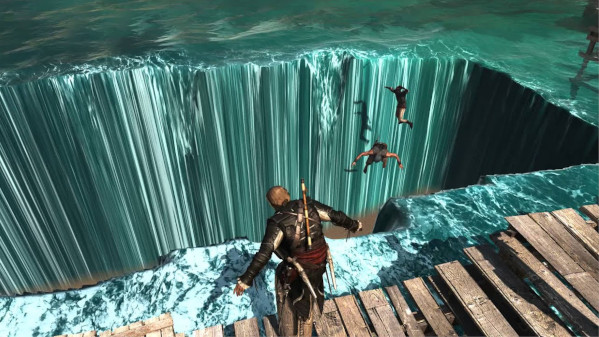
\includegraphics{figures/black_flag_not_water_simulation.jpg}
            \captionof{figure}{Assassin's Creed: Black Flag - Pas de simulation de fluide}
            \label{fig:test1}
        \end{minipage}%
        \begin{minipage}{.5\textwidth}
            \centering
            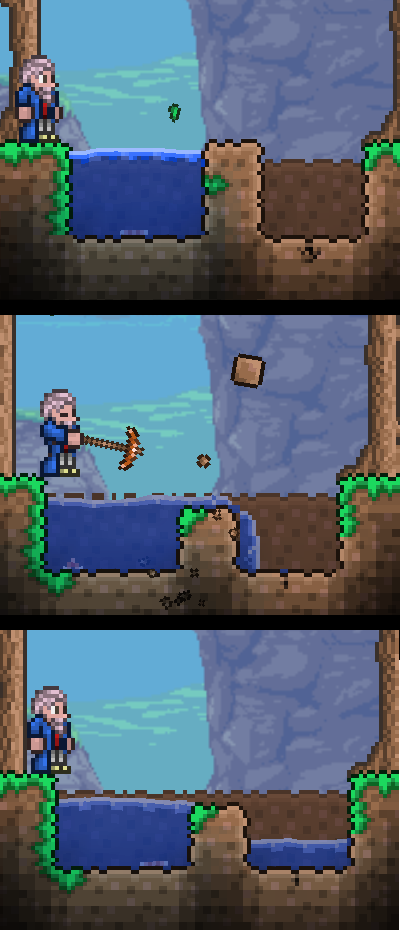
\includegraphics[height=6cm]{figures/terrarria_fluid_sim.png}
            \captionof{figure}{Terrarria - Simulation de fluide}
            \label{fig:test2}
        \end{minipage}
    \end{figure}
\end{frame}

% La table des matières utilise ce que vous donnez aux commandes \section et 
% \subsection tout au long de la présentation.
\begin{frame}
\frametitle{Plan de l'exposé} 
\tableofcontents 
\end{frame}


% La première grande partie: introduction du sujet
% Titre de la premiere partie
\section{\fstpti}

%%%%%%%%%%%%%%%%%%%%%%%%%%%%%%%%%%%%%%%%%%%%%%%%
% Première diapo
%%%%%%%%%%%%%%%%%%%%%%%%%%%%%%%%%%%%%%%%%%%%%%%%
\begin{frame}
\frametitle{\fstpti}
\framesubtitle{Deux points de vue}

\begin{figure}
	\centering
	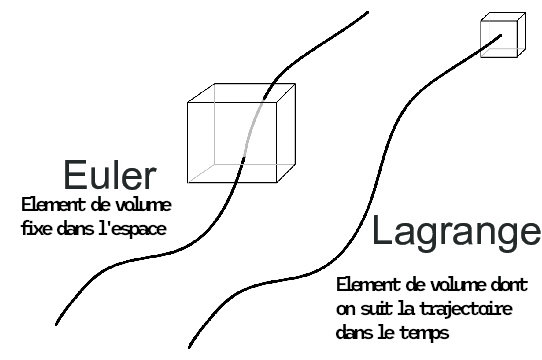
\includegraphics[width=0.8\linewidth]{figures/eulerian_vs_lagrangian_description.png}
\end{figure}

\end{frame}


%%%%%%%%%%%%%%%%%%%%%%%%%%%%%%%%%%%%%%%%%%%%%%%%
% Deuxième diapo
%%%%%%%%%%%%%%%%%%%%%%%%%%%%%%%%%%%%%%%%%%%%%%%%
\begin{frame}
\frametitle{\fstpti}
\framesubtitle{La description Eulerienne}

\noindent
\begin{minipage}[t]{0.6\textwidth}
	Caractéristiques:
	\begin{itemize}
		\item Élément de volume fixe dans l'espace
		\item Les variables d'intéret sont de la forme: $A(M,t)$
	\end{itemize}
\end{minipage}%
\begin{minipage}[t]{0.4\textwidth}
	\adjustimage{width=1.0\textwidth,valign=t}{figures/eulerian_representation.png}
\end{minipage}


\end{frame}


%%%%%%%%%%%%%%%%%%%%%%%%%%%%%%%%%%%%%%%%%%%%%%%%
% Troisième diapo
%%%%%%%%%%%%%%%%%%%%%%%%%%%%%%%%%%%%%%%%%%%%%%%%
\begin{frame}
\frametitle{\fstpti}
\framesubtitle{La description Lagrangienne}

\noindent
\begin{minipage}[t]{0.6\textwidth}
	Caractéristiques:
	\begin{itemize}
		\item Élément de volume bouge dans l'espace
		\item Les variables d'intéret sont de la forme: $A(M_0,t)$
	\end{itemize}
\end{minipage}%
\begin{minipage}[t]{0.4\textwidth}
	\adjustimage{width=1.0\textwidth,valign=t}{figures/lagrangian_representation.png}
\end{minipage}

\end{frame}


%%%%%%%%%%%%%%%%%%%%%%%%%%%%%%%%%%%%%%%%%%%%%%%%
% Quatrième diapo
%%%%%%%%%%%%%%%%%%%%%%%%%%%%%%%%%%%%%%%%%%%%%%%%
\begin{frame}
	\frametitle{\fstpti}
	\framesubtitle{Choix pour mon projet}

	\noindent
	\begin{minipage}[t]{0.5\textwidth}
		Eulerienne:
		\begin{itemize}
			\item Préférée pour la résolution des équations de Navier-Stokes
			\item Préférée pour modélisation de grands systèmes fluides
		\end{itemize}

	\end{minipage}%
	\begin{minipage}[t]{0.5\textwidth}
		Lagrangienne:
		\begin{itemize}
			\item Utile pour des problèmes où les trajectoires des particules sont cruciales
			\item Par exemple la simulation des mouvements de particules de fluide
		\end{itemize}

	\end{minipage}
	\newline
	\newline
	\newline
	\begin{minipage}[b]{0.5\textwidth}
		\textcolor{red}{\xmark} Utilisation non pertinente
	\end{minipage}%	
	\begin{minipage}[b]{0.5\textwidth}
		\textcolor{green}{\cmark} Utilisation pertinente
	\end{minipage}%


\end{frame}

%%%%%%%%%%%%%%%%%%%%%%%%%%%%%%%%%%%%%%%%%%%%%%%%
% Cinquieme diapo
%%%%%%%%%%%%%%%%%%%%%%%%%%%%%%%%%%%%%%%%%%%%%%%%
\begin{frame}
	\frametitle{\fstpti}
	\framesubtitle{Les équations du mouvement d'une particule de fluide}

	Pour une particule de fluide de volume $d\tau$ de masse $m$ et de masse volumique $\rho$, la 2nde loi de newton s'écrit:
	\begin{align*}
	m \frac{d\vec{v}}{dt} &= \vec{F}_{contact} + \vec{F}_{distance}
	\end{align*}

\end{frame}

%%%%%%%%%%%%%%%%%%%%%%%%%%%%%%%%%%%%%%%%%%%%%%%%
% Sixieme diapo
%%%%%%%%%%%%%%%%%%%%%%%%%%%%%%%%%%%%%%%%%%%%%%%%
\begin{frame}
	\frametitle{\fstpti}
	\framesubtitle{Les forces à distance}
	Forces à distances:
	\begin{itemize}
		\item Le poids: $\vec{P} = m \vec{g} = \rho d\tau \vec{g}$ 
		\item La force de Lorentz: $\vec{F_L} = q(\vec{E} + \vec{v}\wedge \vec{B}) = \vec{0}$
	\end{itemize}
	
	\hfill

	
	Expression:
	\begin{align*}
		\Aboxed{\vec{F}_{distance} = \rho d\tau \vec{g}}
	\end{align*}

\end{frame}

%%%%%%%%%%%%%%%%%%%%%%%%%%%%%%%%%%%%%%%%%%%%%%%%
% Septieme diapo
%%%%%%%%%%%%%%%%%%%%%%%%%%%%%%%%%%%%%%%%%%%%%%%%
\begin{frame}
	\frametitle{\fstpti}
	\framesubtitle{Les forces de contact}

	\noindent
	\begin{minipage}[t]{0.6\textwidth}
		Décomposition de la force de contact
		\begin{align*}
			d\vec{F}_{contact} = \underbrace{d\vec{F}_{tangentielle}}_\text{Viscosite} 	+ \underbrace{d\vec{F}_{normale}}_\text{Pression}
		\end{align*}
	\end{minipage}%
	\begin{minipage}[t]{0.4\textwidth}
		\adjustimage{width=1.0\textwidth,valign=t}{figures/force_de_contact_particule_de_fluide.png}
	\end{minipage}

	Après calculs on obtient les expressions suivantes:

	\noindent
	\begin{minipage}[t]{0.5\textwidth}
		\begin{align*}
			\Aboxed{d\vec{F}_{pression} = -\vec{\text{grad}}(P)d\tau}
		\end{align*}
	\end{minipage}%
	\begin{minipage}[t]{0.5\textwidth}
		\begin{align*}
			\Aboxed{d\vec{F}_{viscosite} = \eta \Delta \vec{v} d\tau}
		\end{align*}
	\end{minipage}

\end{frame}

%%%%%%%%%%%%%%%%%%%%%%%%%%%%%%%%%%%%%%%%%%%%%%%%
% Huitième diapo
%%%%%%%%%%%%%%%%%%%%%%%%%%%%%%%%%%%%%%%%%%%%%%%%

\begin{frame}
	\frametitle{\fstpti}
	\framesubtitle{Les équations de Navier-Stokes}
	
	Équation de conservation de la quantité de mouvement:
	\begin{align*}
		\Aboxed{\rho \Big [\frac{\partial \vec{v}}{\partial t} +\vec{v} \cdot \vec{\text{grad}}(v) \Big ]= \rho \vec{g} - \vec{grad} P + \eta \Delta \vec{v} + \vec{F}}
	\end{align*}

	Équation de conservation de la masse:
	\begin{align*}
		\Aboxed{\frac{\partial \rho}{\partial t} + \rho \text{div } \vec{v} = 0}
	\end{align*}

\end{frame}


% La 2e partie: Le point de vue de la relativité restreinte
% Titre de la partie
\section{\sndpti}

%%%%%%%%%%%%%%%%%%%%%%%%%%%%%%%%%%%%%%%%%%%%%%%%
% Première diapo
%%%%%%%%%%%%%%%%%%%%%%%%%%%%%%%%%%%%%%%%%%%%%%%%
\begin{frame}
\frametitle{\sndpti}
\framesubtitle{Méthode SPH}

\centering {\huge \sndpti}

\end{frame}


%%%%%%%%%%%%%%%%%%%%%%%%%%%%%%%%%%%%%%%%%%%%%%%%
% Deuxième diapo
%%%%%%%%%%%%%%%%%%%%%%%%%%%%%%%%%%%%%%%%%%%%%%%%
\begin{frame}
\frametitle{\sndpti}
\framesubtitle{Méthode SPH}

\centering
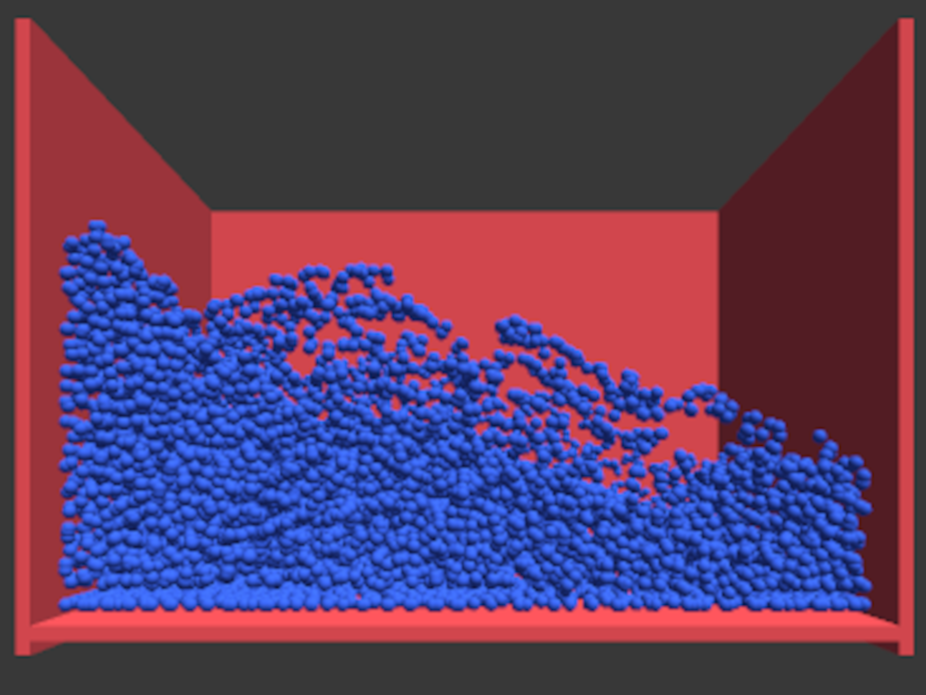
\includegraphics[width=.7\linewidth]{figures/sph_illustration.png}

\end{frame}

%%%%%%%%%%%%%%%%%%%%%%%%%%%%%%%%%%%%%%%%%%%%%%%%
% Troisième diapo
%%%%%%%%%%%%%%%%%%%%%%%%%%%%%%%%%%%%%%%%%%%%%%%%
\begin{frame}
\frametitle{\sndpti}
\framesubtitle{Avantages de cette technique}

\begin{itemize}
    \item Respect de l'équation de conservation de la masse
    \item le terme d'advection est nul 
\end{itemize}
$$(\vec{v}\cdot \vec{\text{grad}}) (\vec{v}) = 0$$

\end{frame}

%%%%%%%%%%%%%%%%%%%%%%%%%%%%%%%%%%%%%%%%%%%%%%%%
% Quatrième diapo
%%%%%%%%%%%%%%%%%%%%%%%%%%%%%%%%%%%%%%%%%%%%%%%%
\begin{frame}
    \frametitle{\sndpti}
    \framesubtitle{Les équations que nous font résoudre cette méthode}
    
    On doit donc juste résoudre:
    $$
    \rho \frac{\partial \vec{v}}{\partial t}= \rho \vec{g} - \vec{grad} P + \eta \Delta \vec{v} + \vec{F}
    $$
    
\end{frame}


%%%%%%%%%%%%%%%%%%%%%%%%%%%%%%%%%%%%%%%%%%%%%%%%
% Cinquieme diapo
%%%%%%%%%%%%%%%%%%%%%%%%%%%%%%%%%%%%%%%%%%%%%%%%
\begin{frame}
    \frametitle{\sndpti}
    \framesubtitle{Obtiention des approximations: prérequis - pseudo-fonction de Dirac}

    \begin{tcolorbox}
        La pseudo-fonction de Dirac:
        \begin{align*}
            \delta(x) =
           \begin{cases}
             + \infty & \text{si } x=0 \\
             0 & \text{sinon}
            \end{cases} \\
            \int_{-\infty}^{+\infty} \delta(x)dx = 1
           \end{align*}
    \end{tcolorbox}

    
\end{frame}


%%%%%%%%%%%%%%%%%%%%%%%%%%%%%%%%%%%%%%%%%%%%%%%%
% Sixième diapo
%%%%%%%%%%%%%%%%%%%%%%%%%%%%%%%%%%%%%%%%%%%%%%%%
\begin{frame}
    \frametitle{\sndpti}
    \framesubtitle{Obtiention des approximations: prérequis - l'identité du Dirac}

    \begin{tcolorbox}
        L'identité du Dirac:

        $\forall g$ continue et intégrable
        \begin{align*}
            \int_\mathbb{R} g(x)\delta(x-t)dx = g(t)
           \end{align*}
    \end{tcolorbox}

\end{frame}

%%%%%%%%%%%%%%%%%%%%%%%%%%%%%%%%%%%%%%%%%%%%%%%%
% Septieme diapo
%%%%%%%%%%%%%%%%%%%%%%%%%%%%%%%%%%%%%%%%%%%%%%%%
\begin{frame}
    \frametitle{\sndpti}
    \framesubtitle{Obtiention des approximations: prérequis - estimation par noyau}
    \onslide*<1>{
        \noindent
        \begin{minipage}[t]{0.4\textwidth}
            Estimation par noyau:
            $$\hat{f}_h(x) = \frac{1}{nh} \sum_{i=1}^n K(\frac{x - x_i}{h})$$
    
            \begin{itemize}
                \item $h$: paramètre de lissage
                \item $K$: fonction noyau de lissage
                \item $n$: nombre de points
               \end{itemize}
        \end{minipage}%
        \begin{minipage}[t]{0.6\textwidth}
            \adjustimage{width=1.0\textwidth,valign=t,margin=2ex 0ex 0ex 0ex}{figures/kernel_smoother_graph.png}
        \end{minipage}
    }

    \onslide*<2>{ \centering 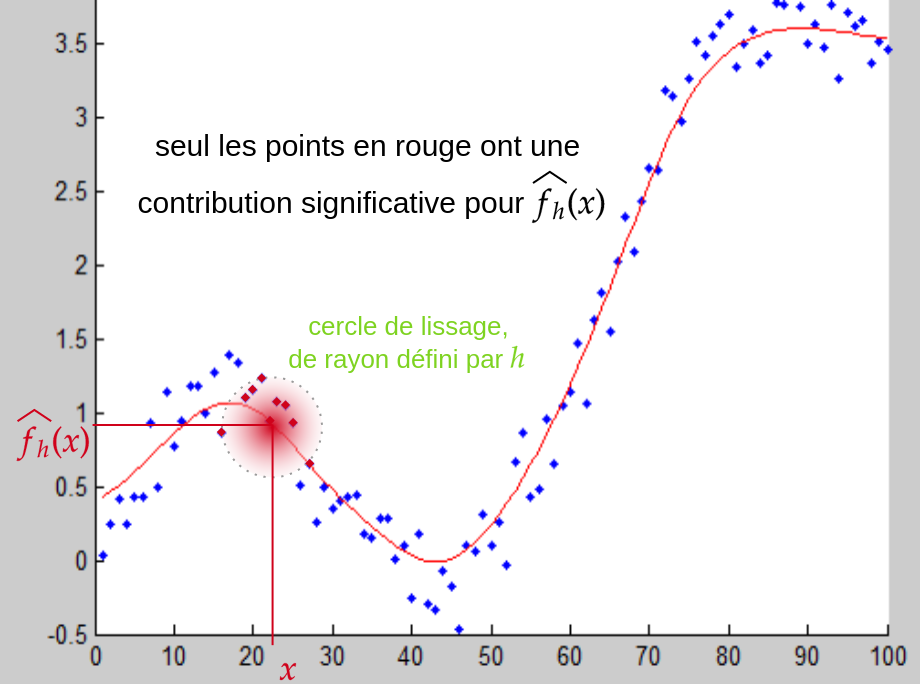
\includegraphics[width=0.8\linewidth]{figures/kernel_smoother_graph.png}}

    \onslide*<3> {
        On pose $\mathbf{q = r/h}$. La fonction $K$ doit répondre à certains critères:
        \begin{align*}
        & \cdot K \text{ positive, définie et décroissante} \\
        & \cdot \lim_{h \to 0}K(r,h) = \delta(r) \\
        & \cdot \sigma \int_{\mathbb{R}^3} f(q)dV = 1
        \end{align*}
    }

\end{frame}

%%%%%%%%%%%%%%%%%%%%%%%%%%%%%%%%%%%%%%%%%%%%%%%%
% Huitieme diapo
%%%%%%%%%%%%%%%%%%%%%%%%%%%%%%%%%%%%%%%%%%%%%%%%
\begin{frame}
    \frametitle{\sndpti}
    \framesubtitle{Expressions dont on doit faire l'approximation}

    \begin{itemize}
        \item<1-> Approximation d'un champs scalaire \\
        \onslide*<2>{
            En posant:
            \begin{align*}
                A(M) = \int_{\mathbb{R}^3} A(M')\delta(\lVert M' - M\rVert)d^3M' \\
                <A>(M) = \int_{\mathbb{R}^3} A(M')K(\lVert M' - M\rVert, h)d^3M'
            \end{align*}
            }
        \onslide*<3>{On se rend compte que:
        \begin{align*}
            A(M) = <A>(M) + O(h^2)
        \end{align*}
        }
        \onslide*<4->{
            \begin{align*}
                A(M) \approx \sum_i \frac{m_i}{\rho_i}A(M_i)K(r_i, h)
            \end{align*}
        }


        \item<5-> Approximation d'un gradient
        \begin{align*}
            \vec{\text{grad}}(A)(M) \approx \sum_i \frac{m_i}{\rho_i}A(M_i) \vec{\text{grad}}(K(r_i, h))
        \end{align*}

        
        \item<6-> Approximation d'un laplacien scalaire
        \begin{align*}
            \Delta A (M) \approx \sum_i \frac{m_i}{\rho_i}A(M_i) \Delta K(r_i, h))
        \end{align*}
    \end{itemize}

\end{frame}

%%%%%%%%%%%%%%%%%%%%%%%%%%%%%%%%%%%%%%%%%%%%%%%%
% Neuvieme diapo
%%%%%%%%%%%%%%%%%%%%%%%%%%%%%%%%%%%%%%%%%%%%%%%%
\begin{frame}
    \frametitle{\sndpti}
    \framesubtitle{Expression discrètes des forces}

    \begin{enumerate}
        \item Densité: $$\rho(M,t) =\sum_i m_i K(r_i, h)$$
        \item Poids: $$\vec{P}(M,t) = \rho(M,t)\vec{g}$$
        \item Pression: $$\vec{F_p}(M,t) = -\sum_i \frac{m_i}{\rho(M_i,t)} p(M_i,t) \vec{\text{grad}}(K(r_i, h))$$
        \item Viscositée: $$\vec{F_{v}}(M,t) = \eta \sum_{j=1}^3 \sum_i m_i \frac{v_i}{\rho(M_i,t)} \Delta K(r_i, h)\vec{u_j}$$
    \end{enumerate}

\end{frame}


% La 3e partie: Le point de vue de la relativité générale
% Le titre de la partie
\section{\trdpti}

%%%%%%%%%%%%%%%%%%%%%%%%%%%%%%%%%%%%%%%%%%%%%%%%
% Première diapo
%%%%%%%%%%%%%%%%%%%%%%%%%%%%%%%%%%%%%%%%%%%%%%%%

\begin{frame}
\frametitle{\trdpti}
\framesubtitle{}

    \centering {\huge \trdpti}

\end{frame}

%%%%%%%%%%%%%%%%%%%%%%%%%%%%%%%%%%%%%%%%%%%%%%%%
% Deuxième diapo
%%%%%%%%%%%%%%%%%%%%%%%%%%%%%%%%%%%%%%%%%%%%%%%%

\begin{frame}
    \frametitle{\trdpti}
    \framesubtitle{Parrallélisme: La carte graphique}
    
    \centering
    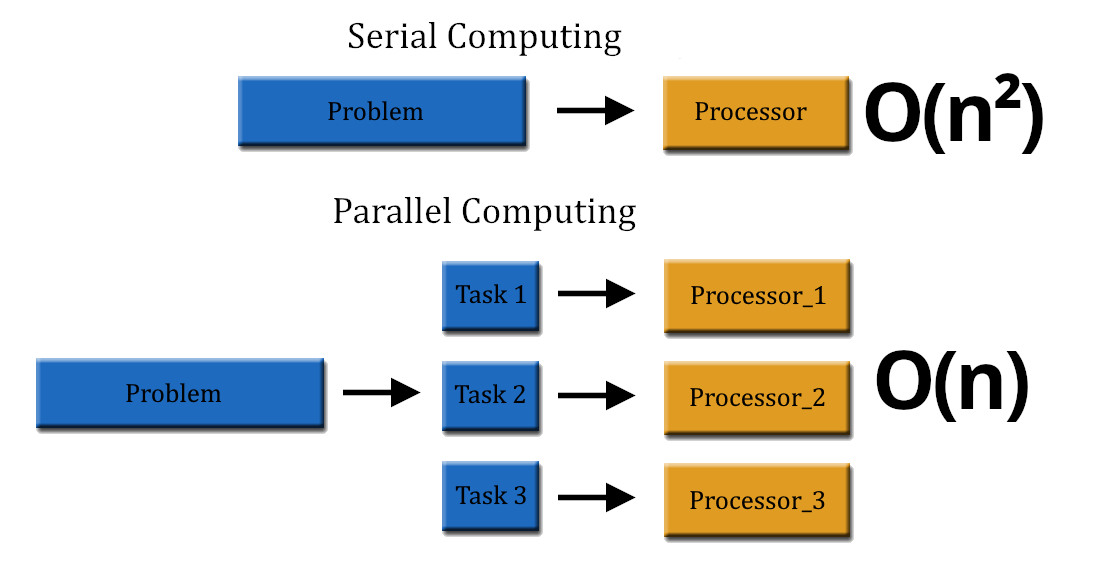
\includegraphics[width=1.0\linewidth]{figures/parallel_computing_vs_sequential_computing.png}
    
\end{frame}


%%%%%%%%%%%%%%%%%%%%%%%%%%%%%%%%%%%%%%%%%%%%%%%%
% Troisième diapo
%%%%%%%%%%%%%%%%%%%%%%%%%%%%%%%%%%%%%%%%%%%%%%%%

\begin{frame}
    \frametitle{\trdpti}
    \framesubtitle{Partitionnement de l'espace}
    
    \centering
    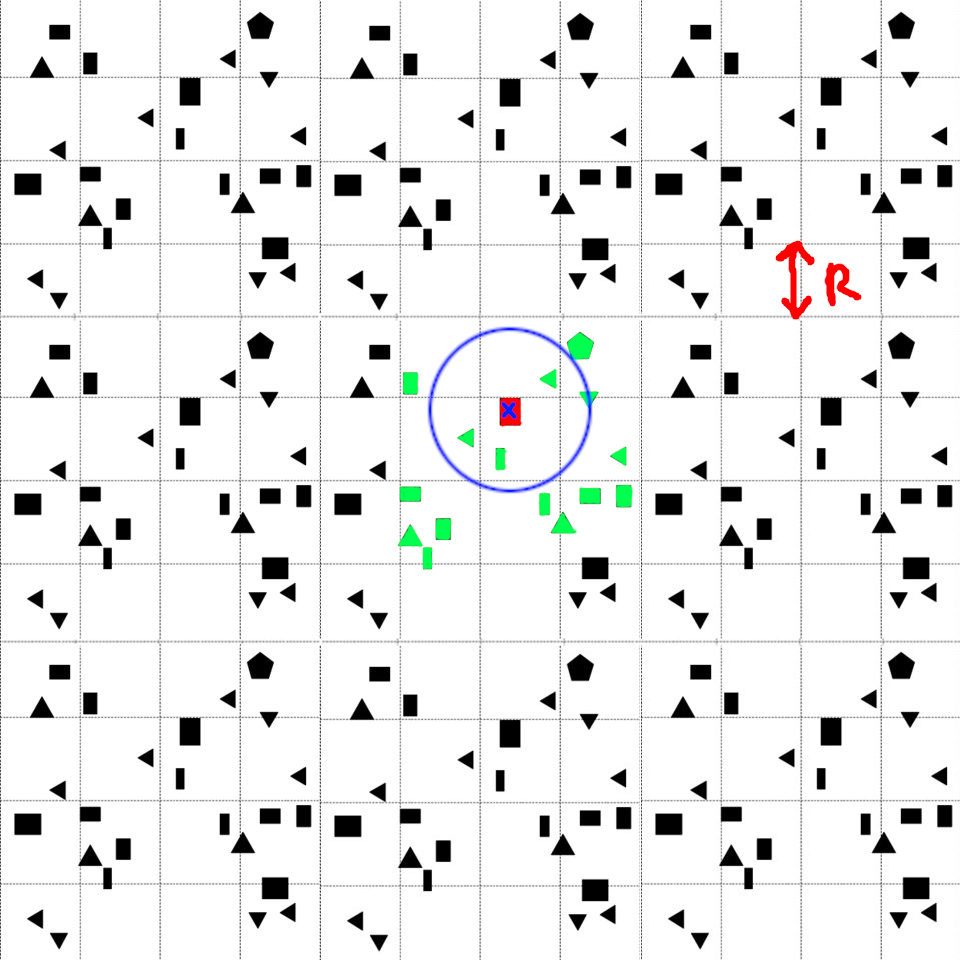
\includegraphics[width=0.75\linewidth]{figures/big_uniform_grid_partitionning.png}
    
\end{frame}


%%%%%%%%%%%%%%%%%%%%%%%%%%%%%%%%%%%%%%%%%%%%%%%%
% Quatrième diapo
%%%%%%%%%%%%%%%%%%%%%%%%%%%%%%%%%%%%%%%%%%%%%%%%

\begin{frame}
    \frametitle{\trdpti}
    \framesubtitle{Explication de l'algorithme de partitionnement}
    
    \onslide*<1-2>{ \centering {\huge
    [\textcolor{red}{0}, \textcolor{red}{1}, \textcolor{red}{2}, \textcolor{red}{3},
     \textcolor{red}{4}, \textcolor{red}{5}, \textcolor{red}{6},
    \textcolor{red}{7}, \textcolor{red}{8}, \textcolor{red}{9}]}}

    \onslide*<3>{ \centering {\huge
    [\textcolor{red}{0}, \textcolor{red}{1}, \textcolor{red}{2}, \textcolor{red}{3},
     \textcolor{red}{4}, \textcolor{red}{5}, \textcolor{red}{6},
    $\overset{\textcolor{red}{7}}{\textcolor{green}{2}}$, \textcolor{red}{8}, \textcolor{red}{9}]}}

    \onslide*<4>{ \centering {\huge
    [
    $\overset{\textcolor{red}{0}}{\textcolor{green}{9}}$,
    $\overset{\textcolor{red}{1}}{\textcolor{green}{0}}$,
    $\overset{\textcolor{red}{2}}{\textcolor{green}{6}}$,
    $\overset{\textcolor{red}{3}}{\textcolor{green}{7}}$,
    $\overset{\textcolor{red}{4}}{\textcolor{green}{1}}$,
    $\overset{\textcolor{red}{5}}{\textcolor{green}{1}}$,
    $\overset{\textcolor{red}{6}}{\textcolor{green}{4}}$,
    $\overset{\textcolor{red}{7}}{\textcolor{green}{2}}$,
    $\overset{\textcolor{red}{8}}{\textcolor{green}{2}}$,
    $\overset{\textcolor{red}{9}}{\textcolor{green}{2}}$
    ]}}

    \onslide*<5>{ \centering Liste spatiale: {\huge
    [
    $\overset{\textcolor{red}{1}}{\textcolor{green}{0}}$,
    $\overset{\textcolor{red}{4}}{\textcolor{green}{1}}$,
    $\overset{\textcolor{red}{5}}{\textcolor{green}{1}}$,
    $\overset{\textcolor{red}{7}}{\textcolor{green}{2}}$,
    $\overset{\textcolor{red}{8}}{\textcolor{green}{2}}$,
    $\overset{\textcolor{red}{9}}{\textcolor{green}{2}}$,
    $\overset{\textcolor{red}{6}}{\textcolor{green}{4}}$,
    $\overset{\textcolor{red}{2}}{\textcolor{green}{6}}$,
    $\overset{\textcolor{red}{3}}{\textcolor{green}{7}}$,
    $\overset{\textcolor{red}{0}}{\textcolor{green}{9}}$
    ]}

    \vspace{10px}

    Liste des départs: {\big [ $0$, $1$, $3$, $+\infty$, $6$, $+\infty$, $8$, $+\infty$, $9$]
    }}

    \onslide*<2-3>{
        \centering
        Indice: 7 \\
        Coordonnées de la case: $(4,1)$ \\
        Hachage des coordonnées: $4532$ \\
        Clé de la cellule: $4532 \mod 10 = 2$
    }

    \onslide*<1->{
        \centering
        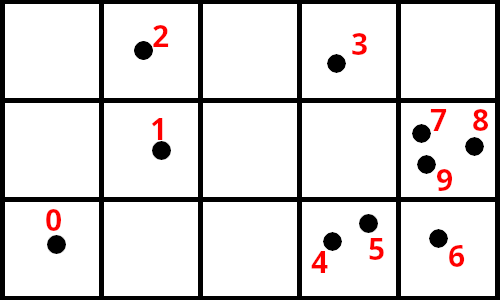
\includegraphics[width=0.5\linewidth]{figures/grid_partitionning_explanation_1.png}
    }
    
\end{frame}

%%%%%%%%%%%%%%%%%%%%%%%%%%%%%%%%%%%%%%%%%%%%%%%%
% Cinquième diapo
%%%%%%%%%%%%%%%%%%%%%%%%%%%%%%%%%%%%%%%%%%%%%%%%

\begin{frame}
    \frametitle{\trdpti}
    \framesubtitle{Tri bitonique}
    
    \centering
    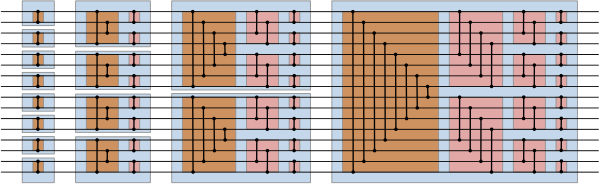
\includegraphics[width=1.0\linewidth]{figures/bitonic_sort.png}
    
\end{frame}


% Conclusion
% Le titre de la partie
\section{\cclpti}

%%%%%%%%%%%%%%%%%%%%%%%%%%%%%%%%%%%%%%%%%%%%%%%%
% Première diapo
%%%%%%%%%%%%%%%%%%%%%%%%%%%%%%%%%%%%%%%%%%%%%%%%
\begin{frame}
    \frametitle{\cclpti}
    \framesubtitle{}
    
    \centering {\huge \cclpti}
    
    \end{frame}

%%%%%%%%%%%%%%%%%%%%%%%%%%%%%%%%%%%%%%%%%%%%%%%%
% Deuxième diapo
%%%%%%%%%%%%%%%%%%%%%%%%%%%%%%%%%%%%%%%%%%%%%%%%
\begin{frame}
    \frametitle{\cclpti}
    \framesubtitle{La simulation}
    
    \centering
    \onslide*<1>{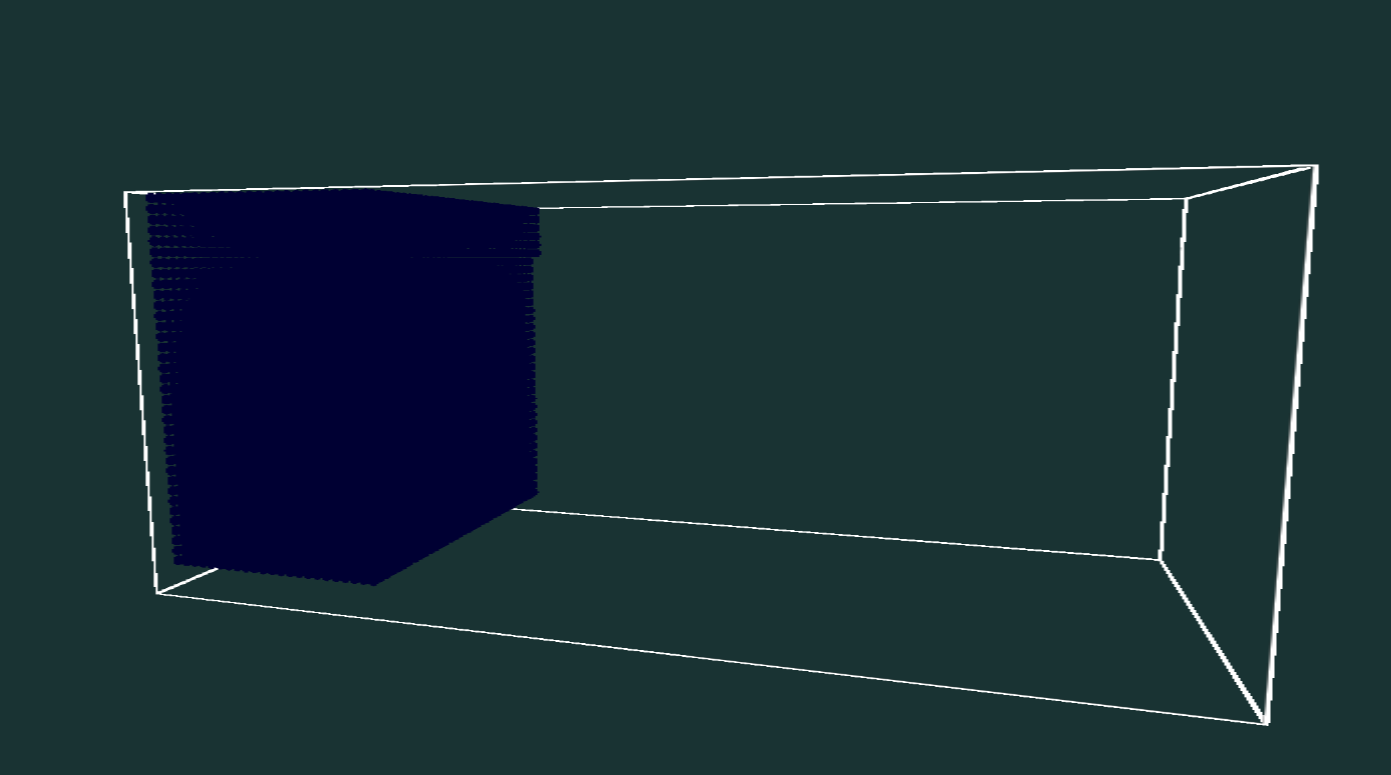
\includegraphics[width=1.0\linewidth]{figures/fluid_sim_finale_1.png}}
    \onslide*<2>{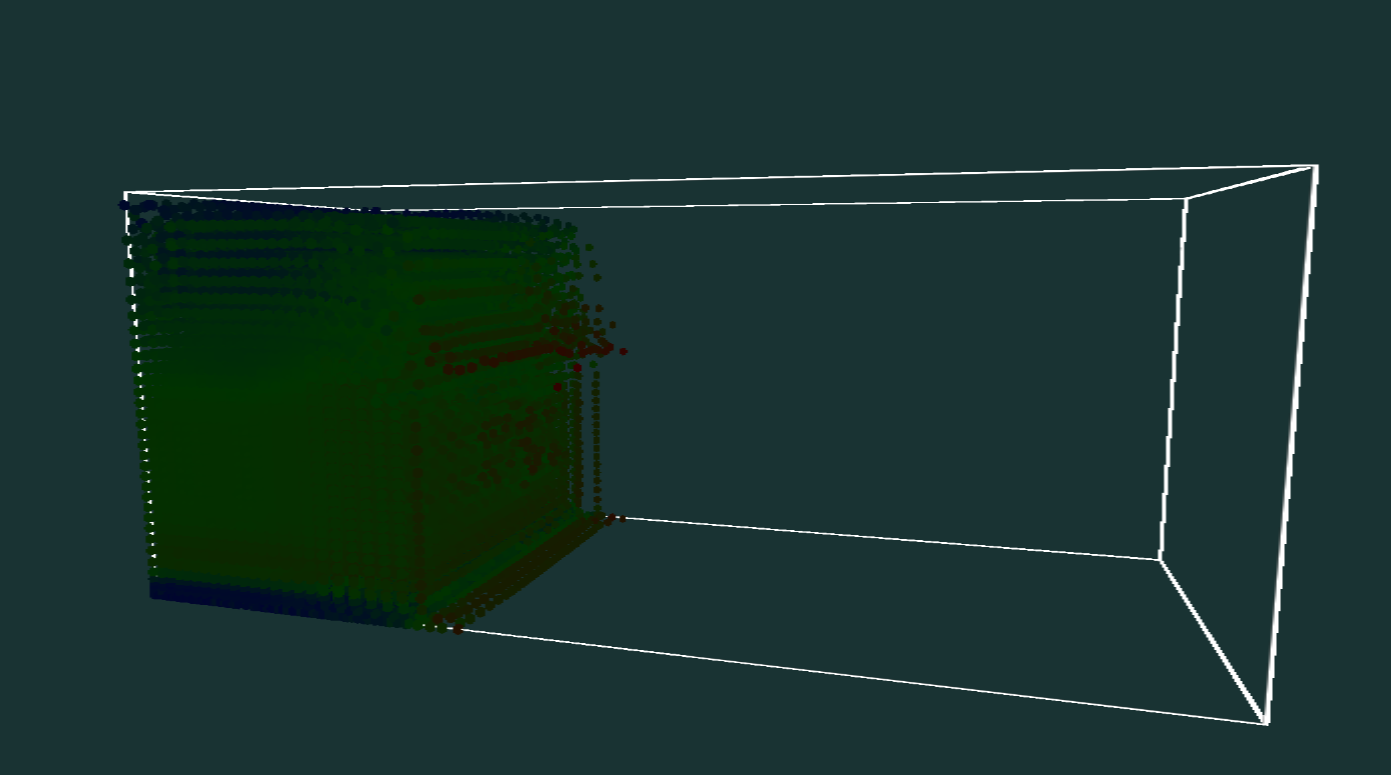
\includegraphics[width=1.0\linewidth]{figures/fluid_sim_finale_2.png}}
    \onslide*<3>{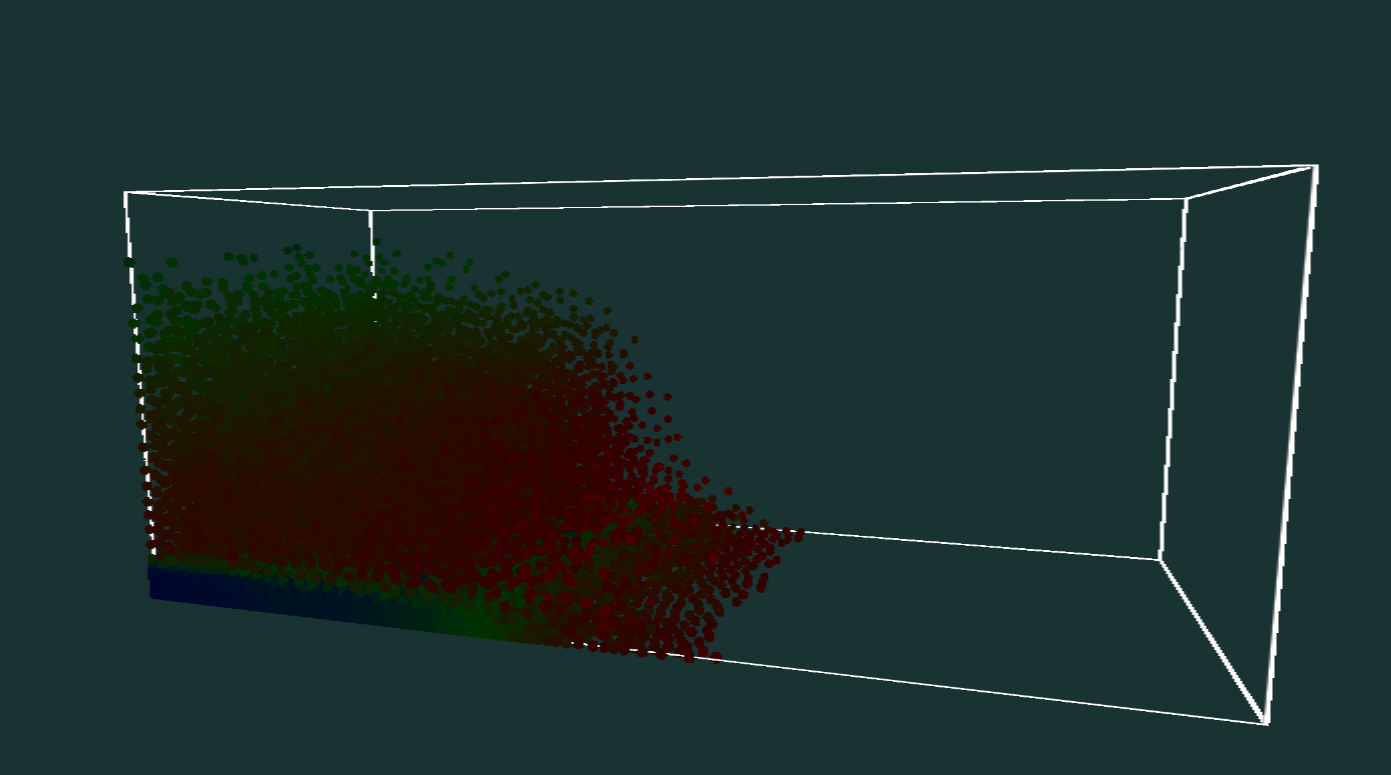
\includegraphics[width=1.0\linewidth]{figures/fluid_sim_finale_3.png}}
    \onslide*<4>{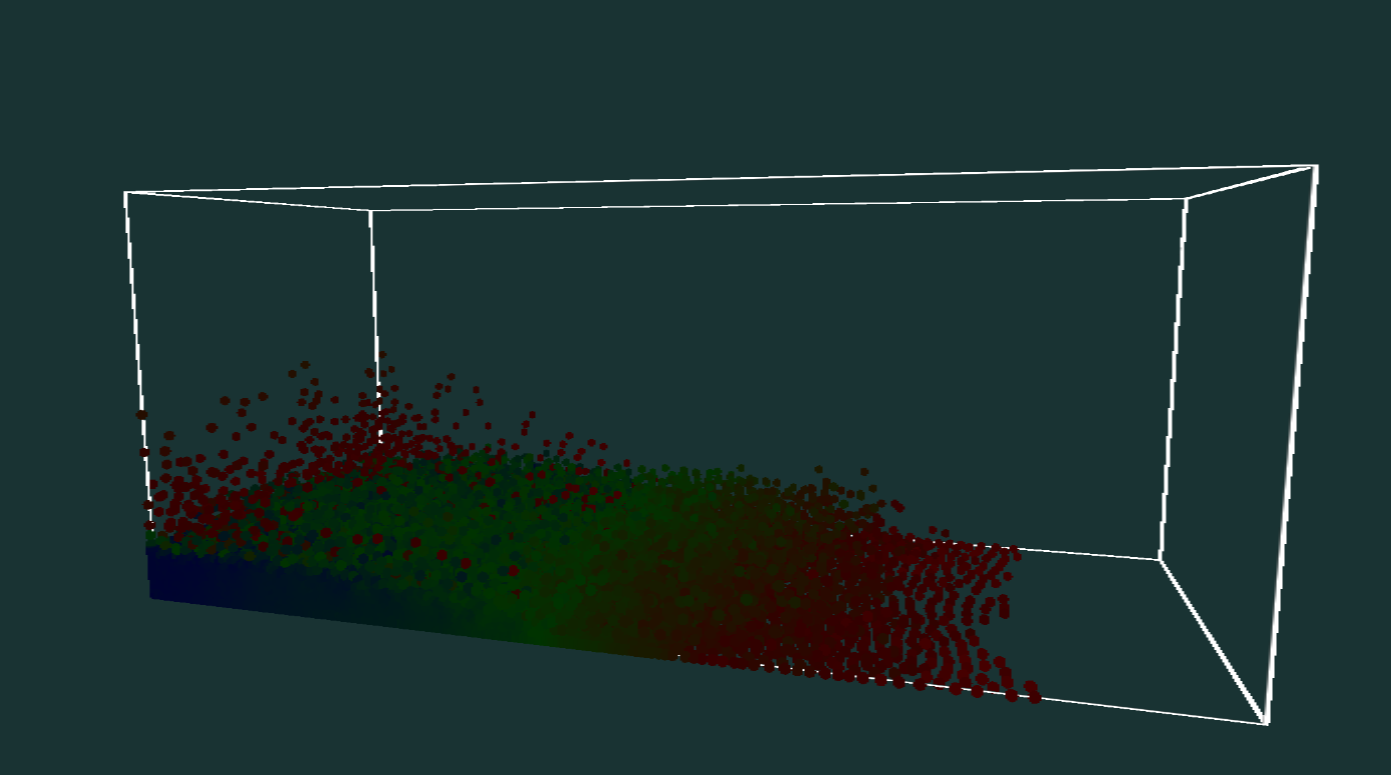
\includegraphics[width=1.0\linewidth]{figures/fluid_sim_finale_4.png}}
    \onslide*<5>{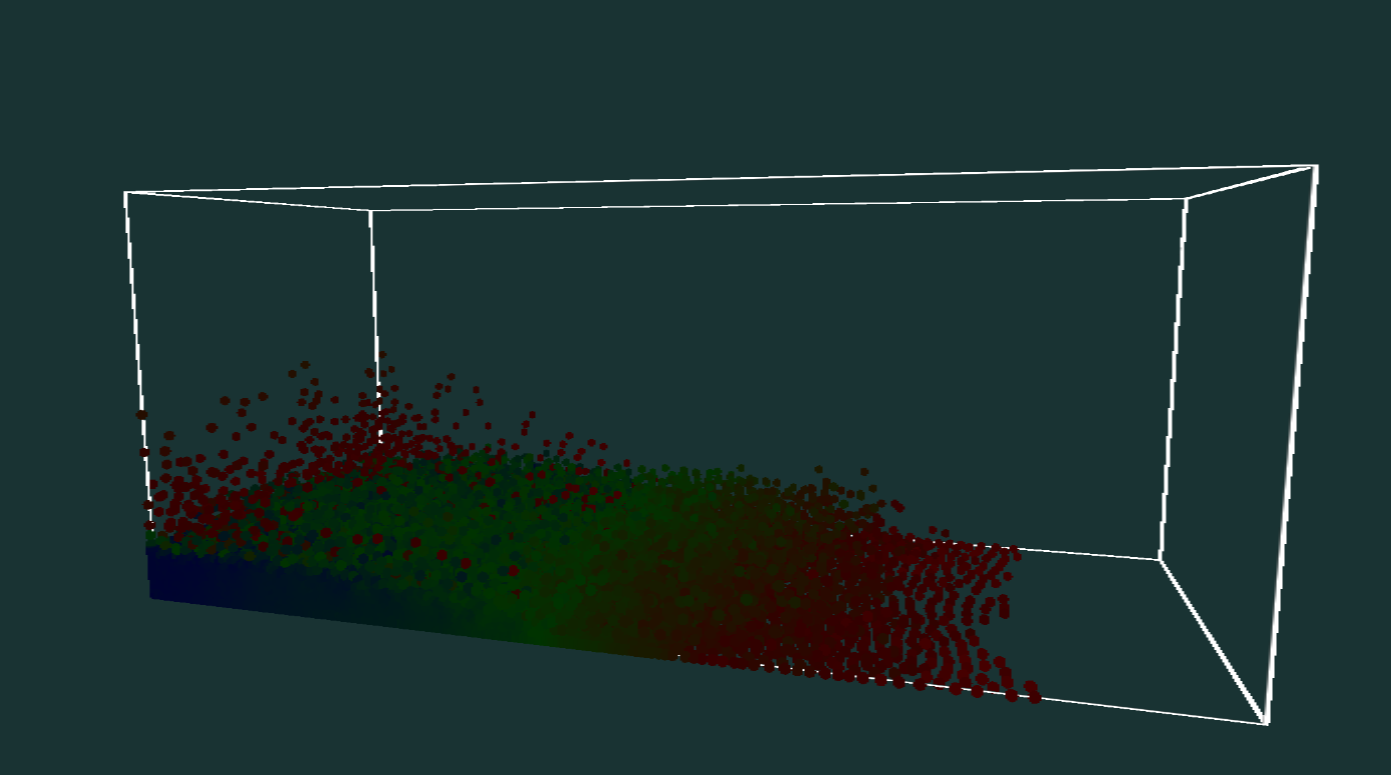
\includegraphics[width=1.0\linewidth]{figures/fluid_sim_finale_5.png}}
    \onslide*<6>{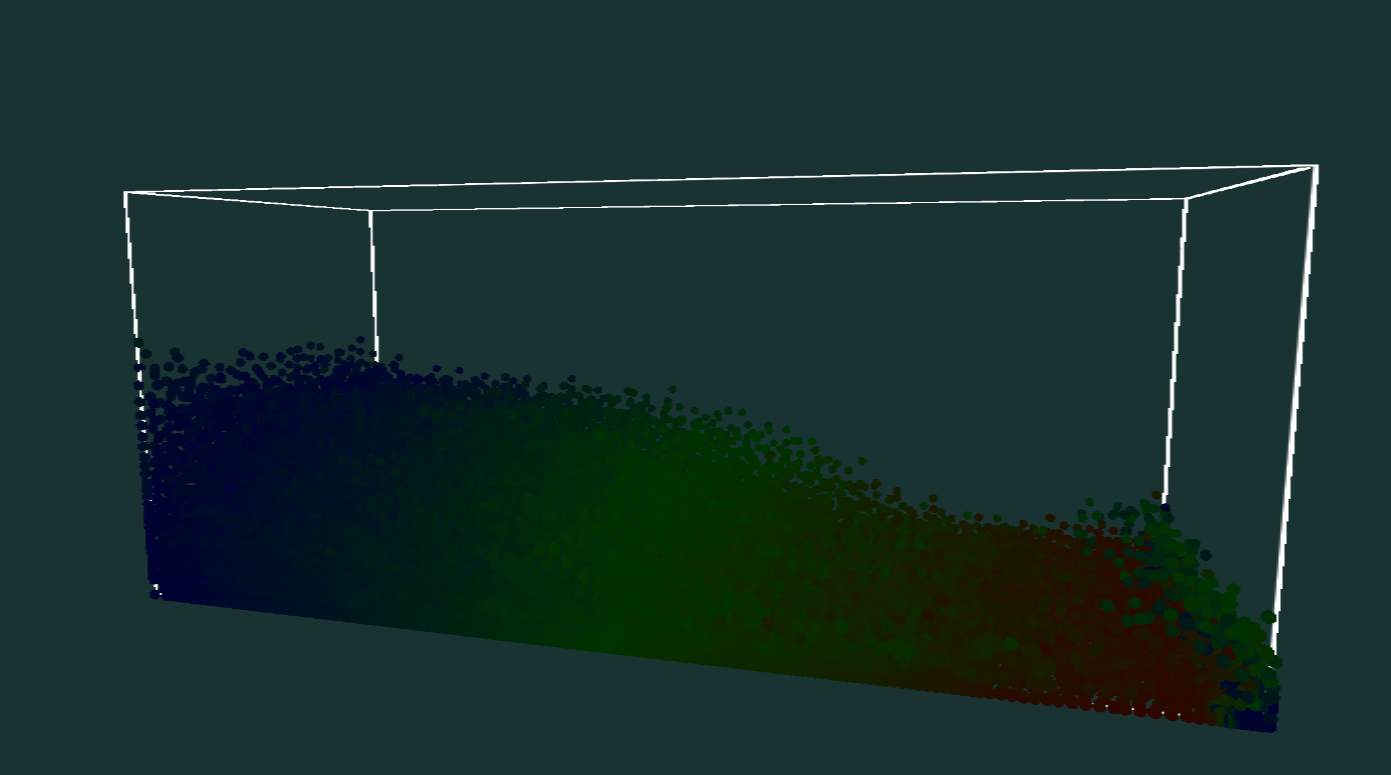
\includegraphics[width=1.0\linewidth]{figures/fluid_sim_finale_6.png}}
    \onslide*<7>{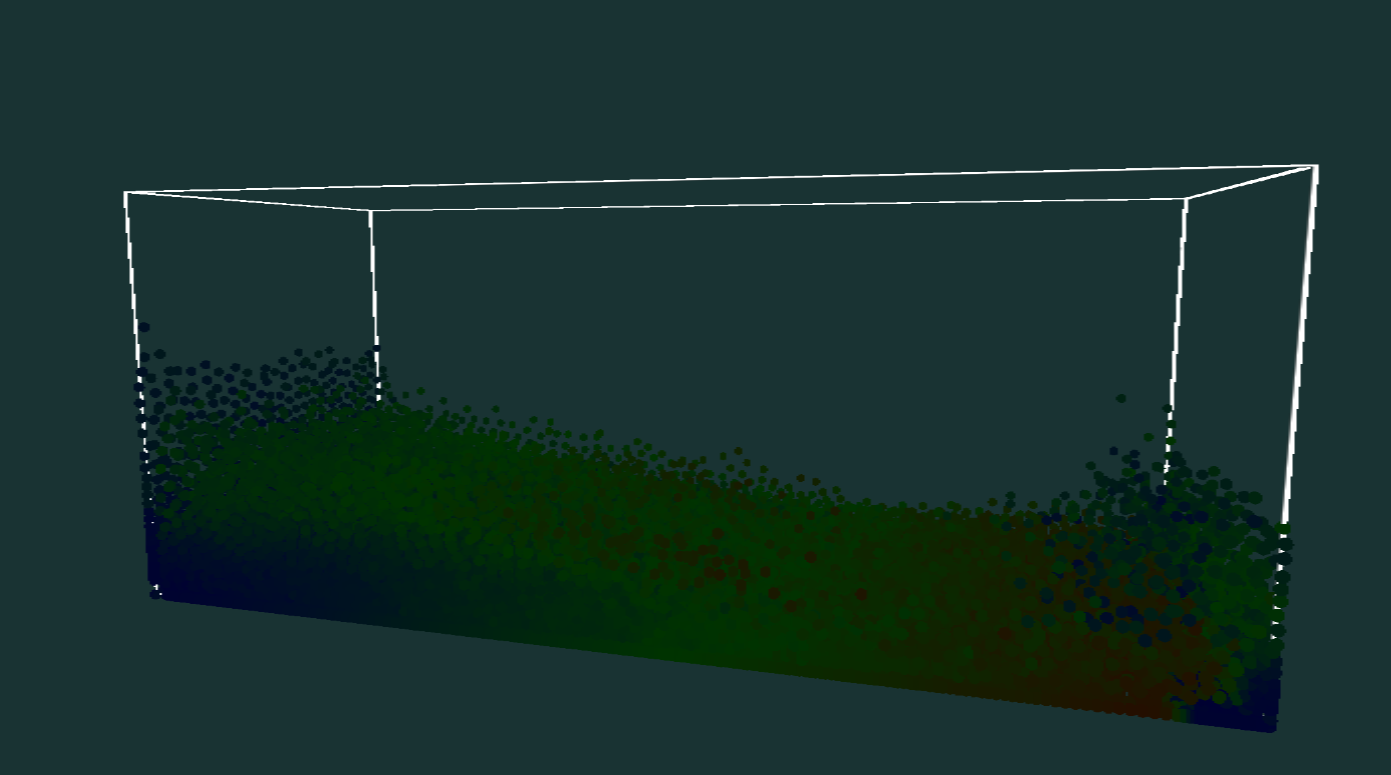
\includegraphics[width=1.0\linewidth]{figures/fluid_sim_finale_7.png}}
    \onslide*<8>{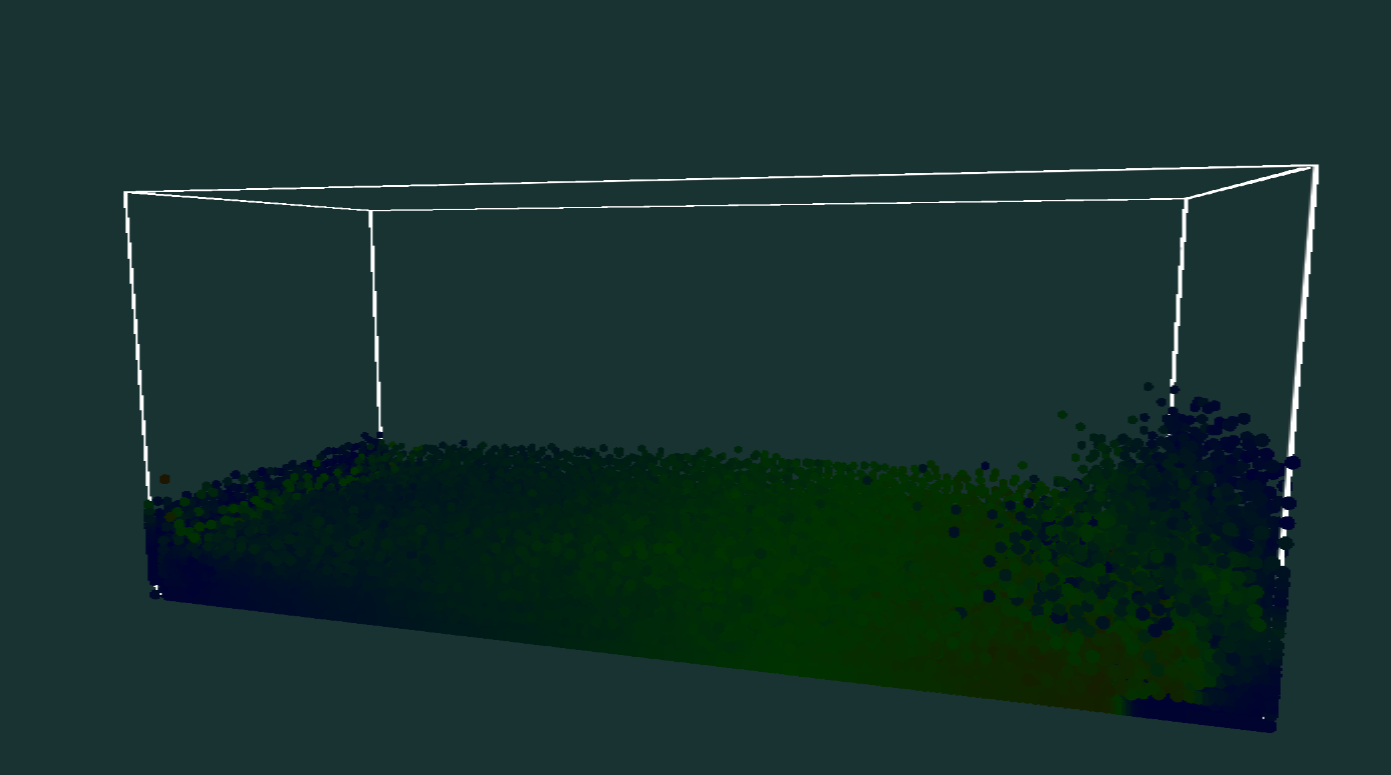
\includegraphics[width=1.0\linewidth]{figures/fluid_sim_finale_8.png}}
    \onslide*<9>{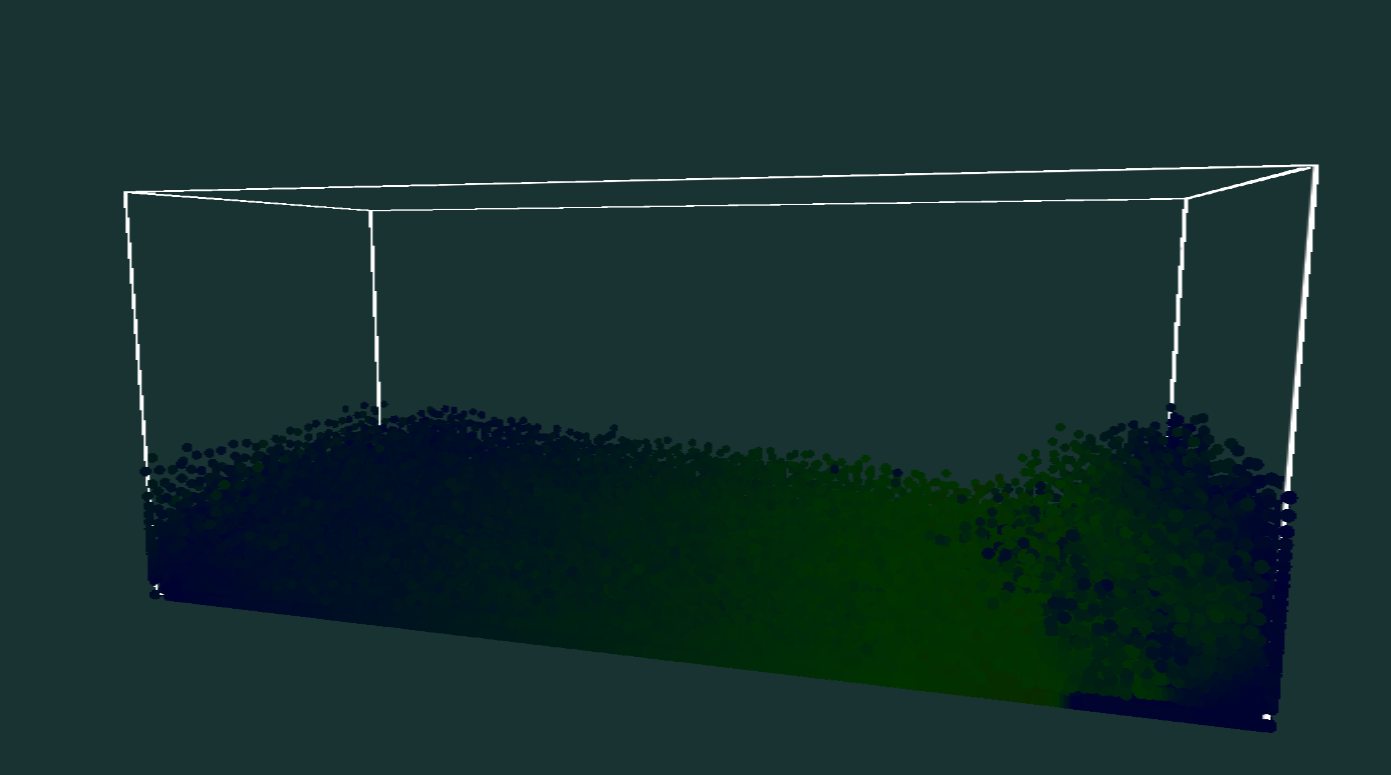
\includegraphics[width=1.0\linewidth]{figures/fluid_sim_finale_9.png}}
    \onslide*<10>{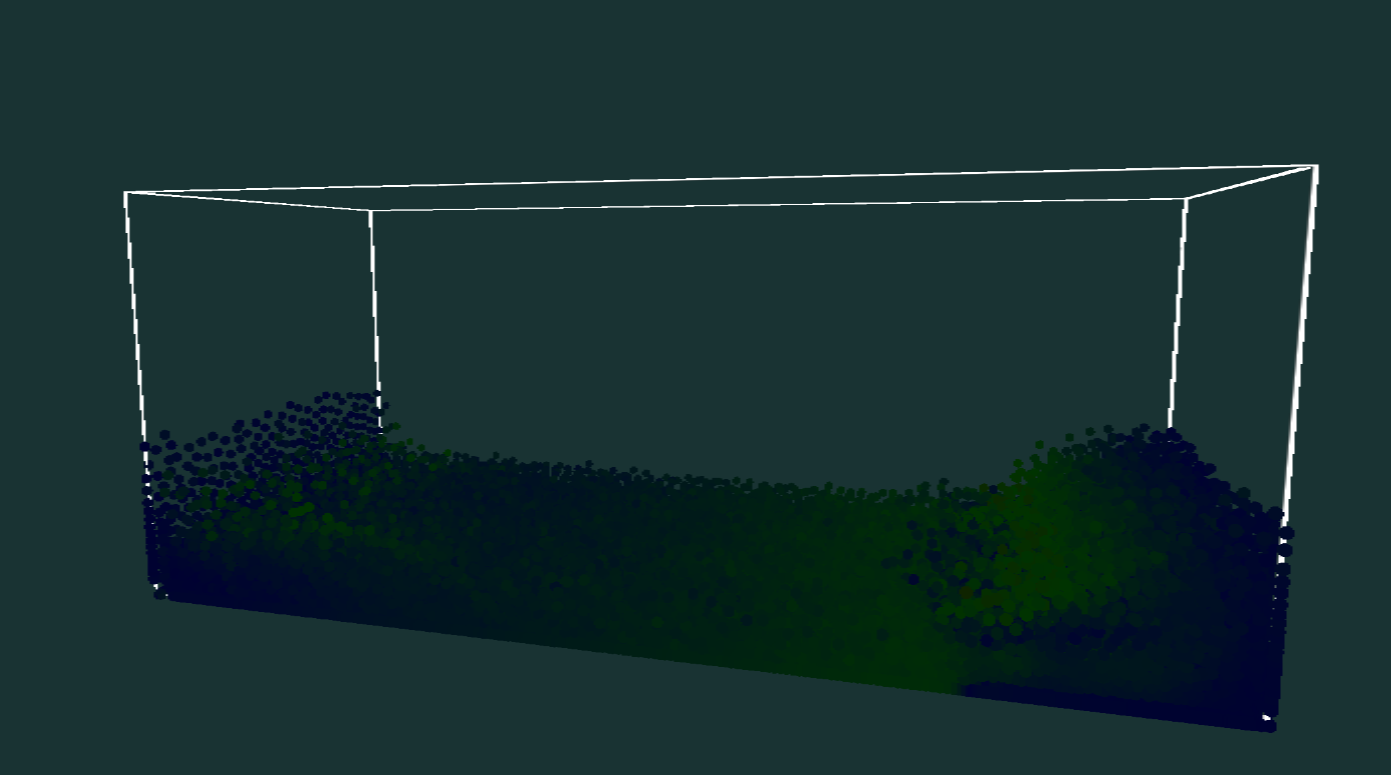
\includegraphics[width=1.0\linewidth]{figures/fluid_sim_finale_10.png}}
    \onslide*<11>{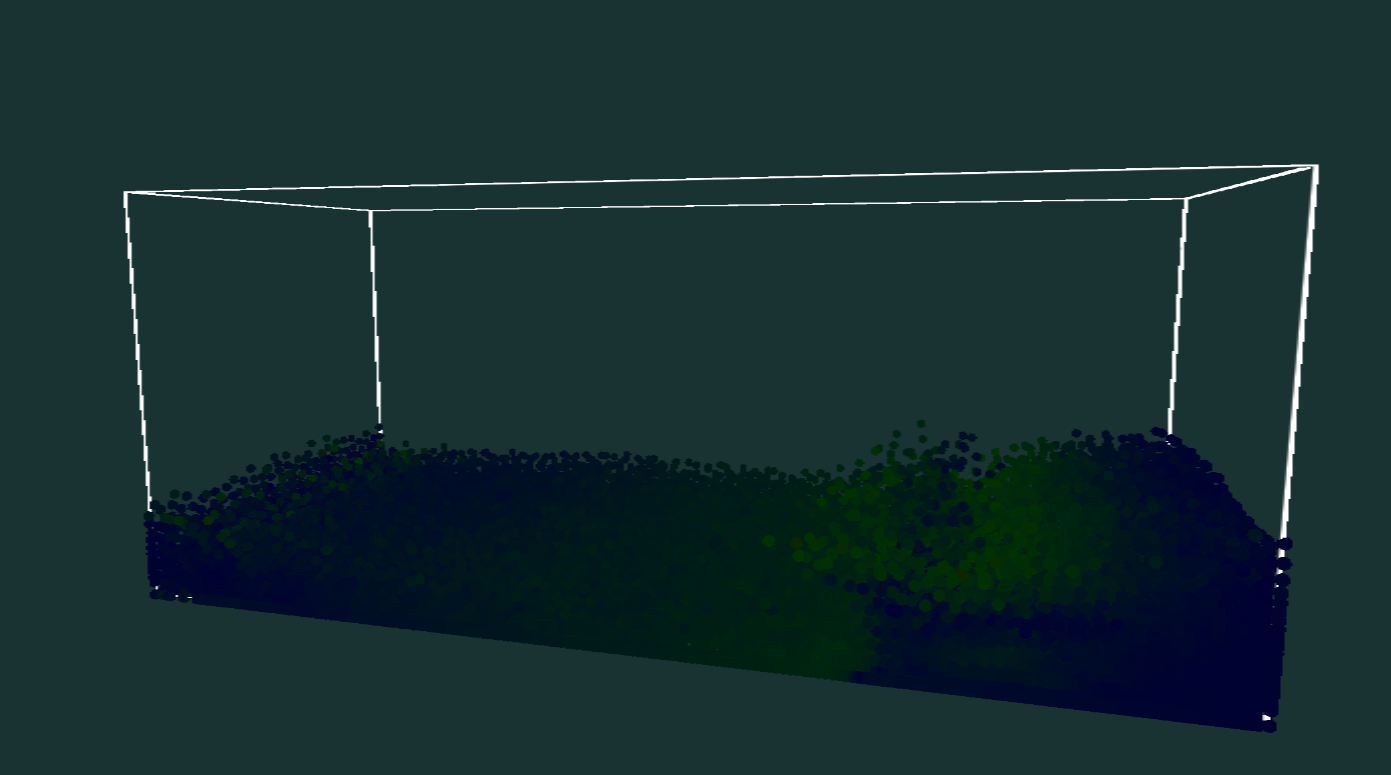
\includegraphics[width=1.0\linewidth]{figures/fluid_sim_finale_11.png}}
    \onslide*<12>{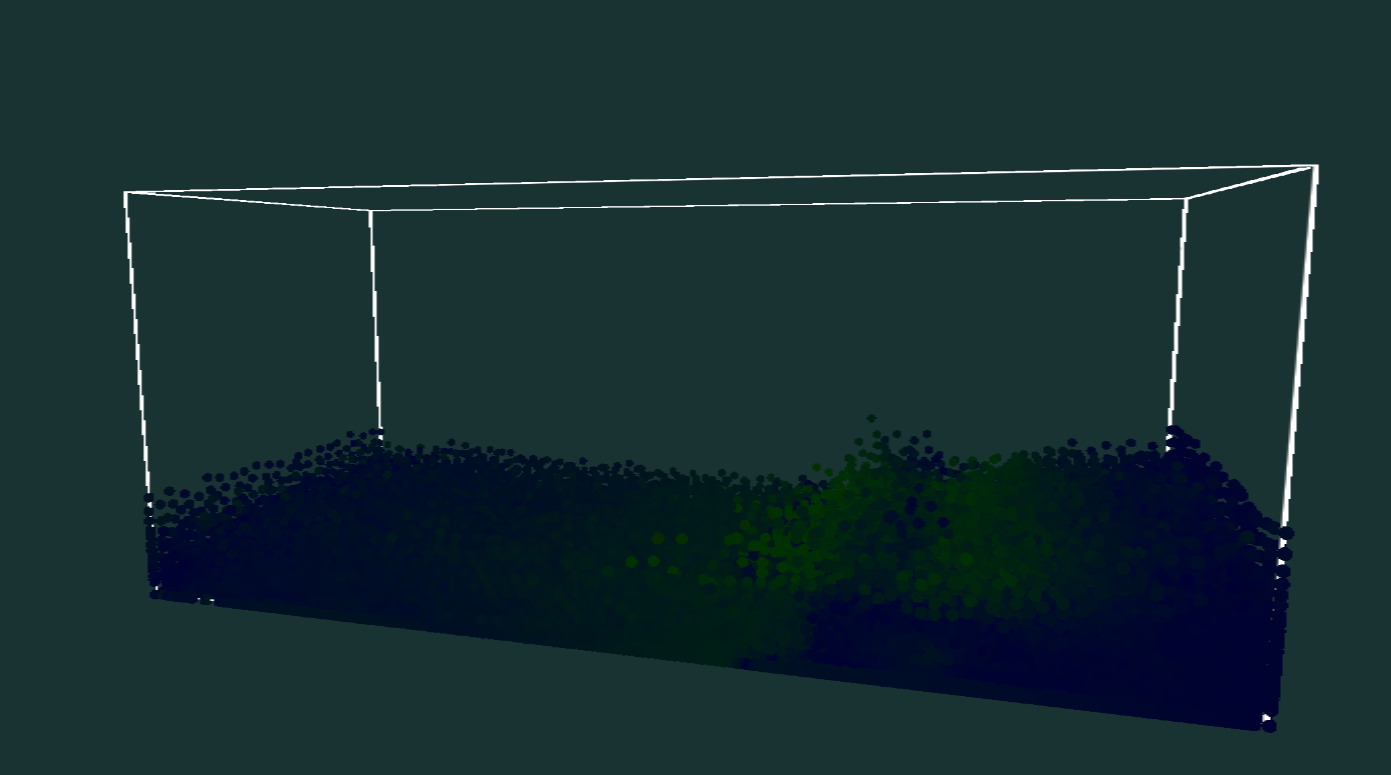
\includegraphics[width=1.0\linewidth]{figures/fluid_sim_finale_12.png}}
    \onslide*<13>{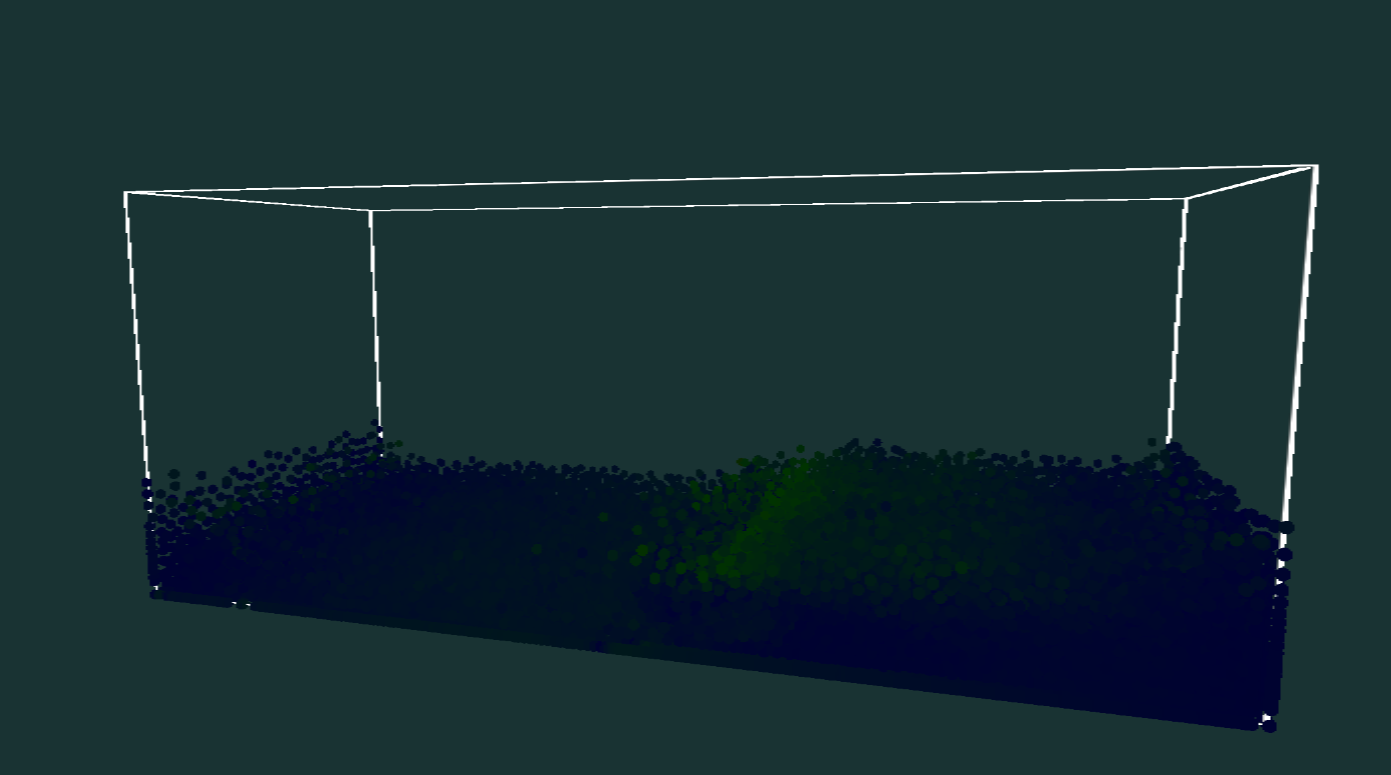
\includegraphics[width=1.0\linewidth]{figures/fluid_sim_finale_13.png}}
    \onslide*<14>{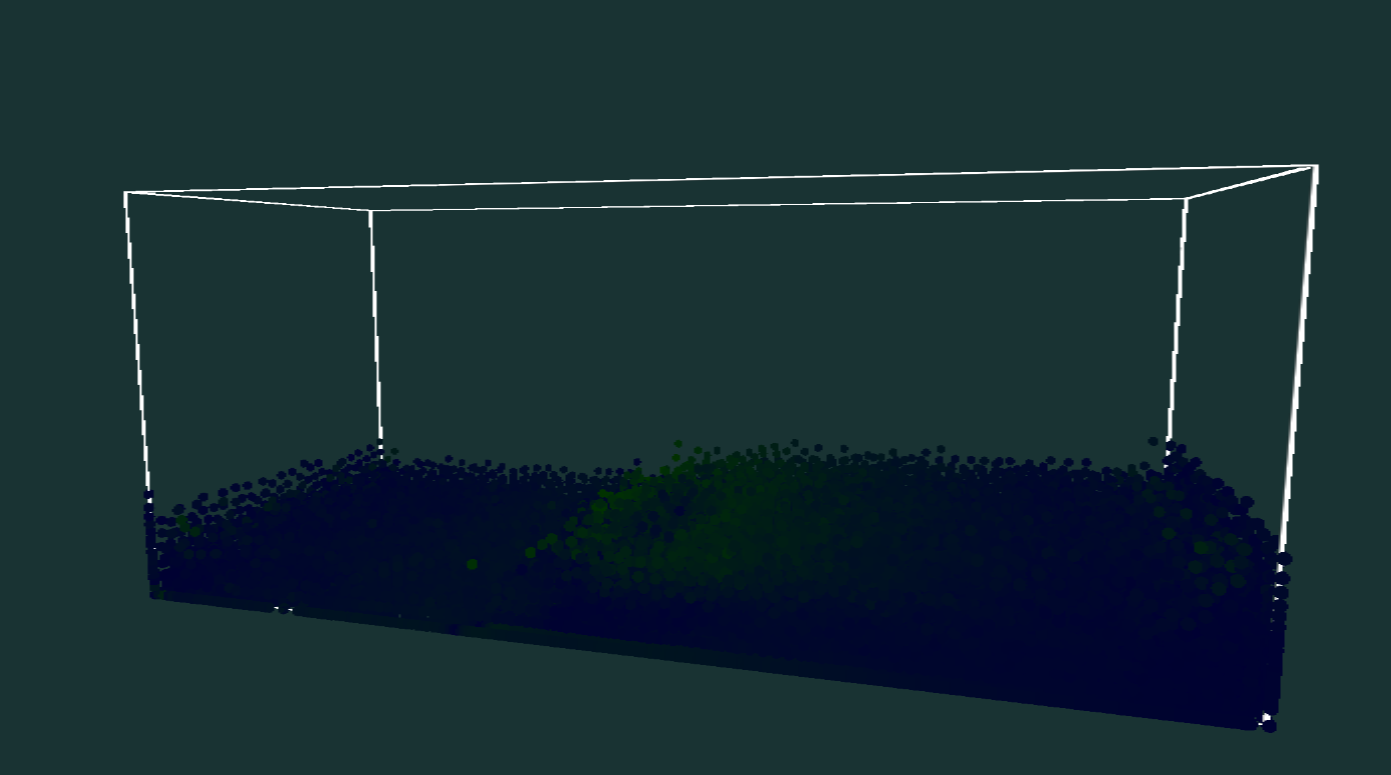
\includegraphics[width=1.0\linewidth]{figures/fluid_sim_finale_14.png}}
    \onslide*<15>{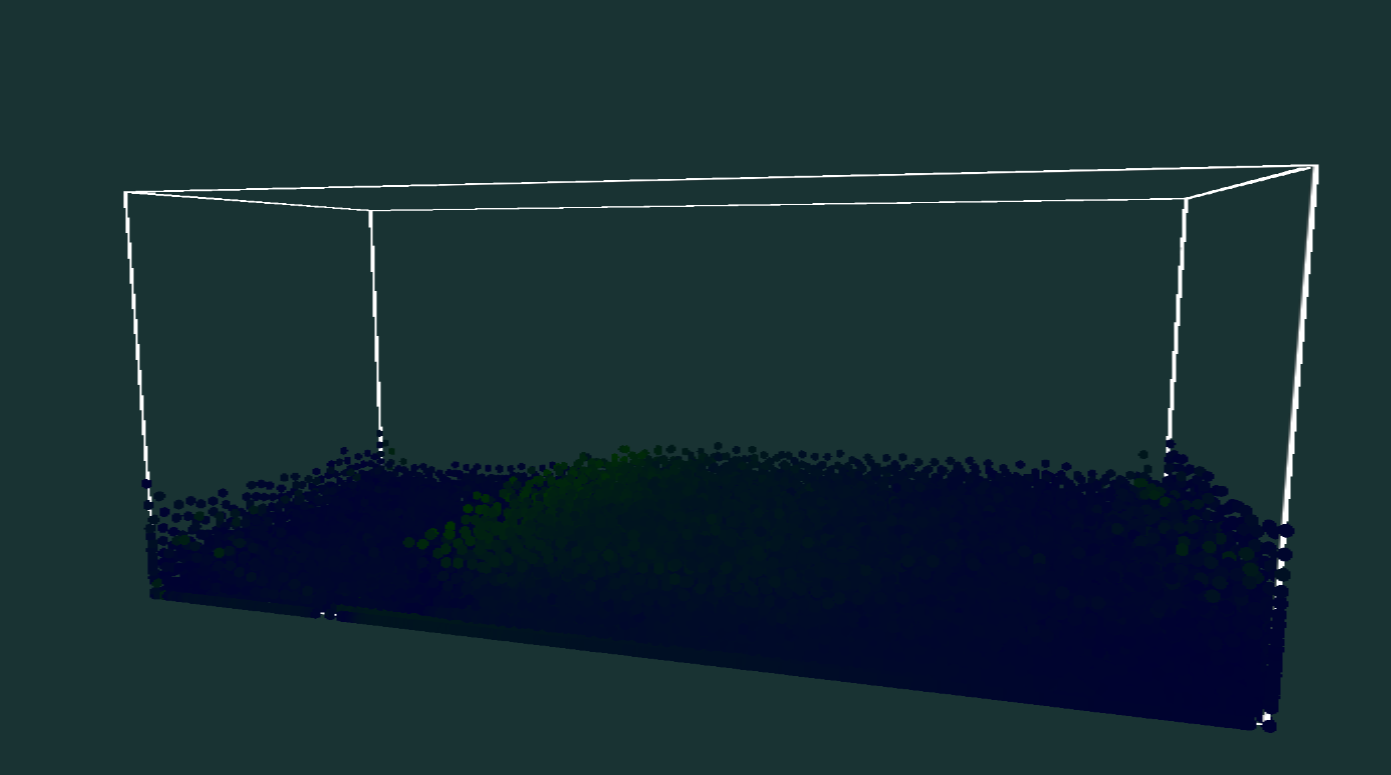
\includegraphics[width=1.0\linewidth]{figures/fluid_sim_finale_15.png}}

\end{frame}

%%%%%%%%%%%%%%%%%%%%%%%%%%%%%%%%%%%%%%%%%%%%%%%%
% 3eme diapo
%%%%%%%%%%%%%%%%%%%%%%%%%%%%%%%%%%%%%%%%%%%%%%%%
\begin{frame}
    \frametitle{\cclpti}
    \framesubtitle{Impact de l'optimisation}
    Nombre de particules maximum pour que la simulation tourne à 60 images par secondes:
    
    \begin{center}
        \begin{tabular}{ |c|c|c| } 
         \hline
         Ajout & Avant & Après \\ 
         \hline
         Passage sur la carte graphique & 350 & 5000 \\ 
         Ajout du partitionnement de l'espace & 5000 & 20.000 \\ 
         Ajout du tri bitonique & 20.000 & 60.000 \\
         \hline
        \end{tabular}
    \end{center}
    
    {\tiny Matériel:
    \begin{itemize}
        \item Processeur: Intel i7-6700 (8) @ 4.0GHz
        \item Carte Graphique: NVIDIA GeForce GTX 1060 6GB
        \item Mémoire Vive: 16Go
    \end{itemize}
    }
    \end{frame}


%Annexe
%%%%%%%%%%%%%%%%%%%%%%%%%%%%%%%%%%%%%%%%%%%%%%%%
% Première diapo
%%%%%%%%%%%%%%%%%%%%%%%%%%%%%%%%%%%%%%%%%%%%%%%%
\begin{frame}
    \frametitle{\anxpti}
    \framesubtitle{}
    
    \centering {\huge \anxpti}
    
    \end{frame}

%%%%%%%%%%%%%%%%%%%%%%%%%%%%%%%%%%%%%%%%%%%%%%%%
% Deuxième diapo
%%%%%%%%%%%%%%%%%%%%%%%%%%%%%%%%%%%%%%%%%%%%%%%%
\begin{frame}[fragile]
    \frametitle{\anxpti}
    \framesubtitle{Code - fluid.py}
    
    \begin{minted}[fontsize=\tiny]{python3}
class Fluid(Entity):
    def __init__(self, particle_count: int, particle_size: float, simulation_corner_1: list[float], simulation_corner_2: list[float], particle_mesh: Mesh = FLUIDPARTICLE_MESH, particle_shaders: Shader = FLUIDPARTICLE_SHADERS) -> None:
        ...
    def init_fluid_shaders(self) -> None:
        ...
    def create_bounding_box(self, scene: Scene) -> tuple[np.ndarray, np.ndarray]:
        ...
    def create_initial_particle_positions(self, position: np.ndarray, scale: np.ndarray) -> np.ndarray:
        ...
    def set_simulation_param(self, name: SimParams, value: any) -> None:
        ...
    def get_simulation_param(self, name: SimParams, from_gpu: bool = False) -> any:
        ...
    def get_buffers(self, binding_point: int, view_as: str = "<f4",start_point: int = 0, size: int = None) -> np.ndarray:
        ...
    def mounted(self, scene: Scene) -> None:
        ...
    def draw(self, scene: Scene)-> None:
        PARTICLEAREA_MATERIAL.use()
        PARTICLEAREA_SHADERS.set_mat4x4("model", self.particle_area.get_model_matrix())
        PARTICLEAREA_MESH.draw()

        self.particle_shaders.set_vec3("camPos", scene.get_camera().get_position())
        self.particle_mesh.prepare_to_draw()
        # On dessine des instances de la particule et non n entités disctinctes pour aller beaucoup plus vite
        glDrawArraysInstanced(GL_TRIANGLES, 0, self.particle_mesh.vertex_count ,self.particle_count)

    \end{minted}
\end{frame}

\begin{frame}[fragile]
    \frametitle{\anxpti}
    \framesubtitle{Code - fluid.py}

    \begin{minted}[fontsize=\tiny]{python3}
    def update(self, delta:float, force_update = False) -> None:
        if self.disable_simulation and not(force_update):
            return 
        
        self.set_simulation_param(SimParams.DELTA, delta)

        self.compute_external.dispatch(self.particle_count)
        self.compute_spatial_hash.dispatch(self.particle_count)
        self.compute_sort.sort_and_calculate_offsets()
        self.compute_density.dispatch(self.particle_count)
        self.compute_pressure.dispatch(self.particle_count)
        self.compute_viscosity.dispatch(self.particle_count)
        self.compute_update_pos.dispatch(self.particle_count)

    def reset_simulation(self, particle_count: int) -> None:
        ...
    def destroy(self) -> None:
        ...
    \end{minted}
\end{frame}


\begin{frame}[fragile]
    \frametitle{\anxpti}
    \framesubtitle{Code - fluid.py}

    \begin{minted}[fontsize=\tiny]{python3}
class GPUSort:
    def __init__(self, index_buffer_size: int) -> None:
        ...
    def next_power_of_2(self, x :int):
        ...
    def sort(self):
        self.sort_shader.set_int("numEntries", self.buffer_size)
        
        num_stages = int(log2(self.next_power_of_2(self.buffer_size)))

        for stage_index in range(num_stages):
            for step_index in range(stage_index + 1):
                # Même chose que 2**(stage_index - step_index) mais beaucoup plus rapide
                groupWidth = 1 << (stage_index - step_index)
                groupHeigth = 2* groupWidth - 1
                self.sort_shader.set_int("groupWidth", groupWidth)
                self.sort_shader.set_int("groupHeight", groupHeigth)
                self.sort_shader.set_int("stepIndex", step_index)

                instances_to_dispatch = self.next_power_of_2(self.buffer_size) // 2
                self.sort_shader.dispatch(instances_to_dispatch)

    def sort_and_calculate_offsets(self):
        self.sort()

        self.offset_shader.set_int("numEntries", self.buffer_size)
        self.offset_shader.dispatch(self.buffer_size)
    \end{minted}
\end{frame}

\begin{frame}[fragile]
    \frametitle{\anxpti}
    \framesubtitle{Code - density.comp}

    \begin{minted}[fontsize=\tiny]{glsl}
void calculateDensities(uint id) {
    if (id >= numParticles) return;
    vec3 pos = predictedPositions[id];
    ivec3 originCell = GetCell3D(pos, smoothingRadius);
    float sqrRadius = smoothingRadius * smoothingRadius;
    float density = 0;
    for (int i = 0; i < 27; i ++) {
        int hash = HashCell3D(originCell + offsets3D[i]);
        int key = KeyFromHash(hash, numParticles);
        uint currIndex = spatialOffsets[key];
        while (currIndex < numParticles) {
            uvec3 indexData = spatialIndices[currIndex];
            currIndex ++;
            if (indexData[2] != key) break;
            if (indexData[1] != hash) continue;
            uint neighbourIndex = indexData[0];
            vec3 neighbourPos = predictedPositions[neighbourIndex];
            vec3 offsetToNeighbour = neighbourPos - pos;
            float sqrDstToNeighbour = dot(offsetToNeighbour, offsetToNeighbour);
            if (sqrDstToNeighbour > sqrRadius) continue;
            float dst = sqrt(sqrDstToNeighbour);
            density += DensityKernel(dst, smoothingRadius);
        }
    }
    densities[id] = density;
}
    \end{minted}
\end{frame}

\begin{frame}[fragile]
    \frametitle{\anxpti}
    \framesubtitle{Code - externalForces.comp}

    \begin{minted}[fontsize=\tiny]{glsl}
void calculateGravity(uint index) {
    if (index >= numParticles) return;

    //Force de gravité
    velocities[index] += vec3(0, gravity, 0) * delta;

    predictedPositions[index] = positions[index] + velocities[index] * delta;
}
    \end{minted}
\end{frame}


\begin{frame}[fragile]
    \frametitle{\anxpti}
    \framesubtitle{Code - gpuSortOffset.comp}

    \begin{minted}[fontsize=\tiny]{glsl}
#version 460 core

layout(binding=5, std430) buffer spatialIndicesBuffer { uvec3 spatialIndices[]; };
layout(binding=6, std430) buffer spatialOffsetsBuffer { uint spatialOffsets[]; };

uniform int numEntries;

layout(local_size_x = 64, local_size_y = 1, local_size_z = 1) in;
void main() {
    uint i = gl_GlobalInvocationID.x;
    
    if (i >= numEntries) { return; }

    uint null = numEntries;

    uint key = spatialIndices[i].z;
    uint keyPrev = i == 0 ? null : spatialIndices[i - 1].z;

    if (key != keyPrev)
    {
        spatialOffsets[key] = i;
    }
}
    \end{minted}
\end{frame}


\begin{frame}[fragile]
    \frametitle{\anxpti}
    \framesubtitle{Code - gpuSort.comp}

    \begin{minted}[fontsize=\tiny]{glsl}
#version 460 core
// le veteur est de la forme (indexe d'origine, hash, clé)
layout(binding=5, std430) buffer spatialIndicesBuffer { uvec3 spatialIndices[]; };
uniform int numEntries;
uniform int groupWidth;
uniform int groupHeight;
uniform int stepIndex;
layout(local_size_x = 64, local_size_y = 1, local_size_z = 1) in;
void main() {
    uint i = gl_GlobalInvocationID.x;
    uint hIndex = i & (groupWidth - 1);
    uint indexLeft = hIndex + (groupHeight + 1) * (i / groupWidth);
    uint rightStepSize = stepIndex == 0 ? groupHeight - 2 * hIndex : (groupHeight + 1) / 2;
    uint indexRight = indexLeft + rightStepSize;
    // S'arrete si on dépasse le nombre de particules à tier (lorsque le nombre de particules n'est pas une puissance de 2)
    if (indexRight >= numEntries) return;
    uint valueLeft = spatialIndices[indexLeft].z;
    uint valueRight = spatialIndices[indexRight].z;
    // On échange les valeurs si elles sont décroissantes
    if (valueLeft > valueRight)
    {
        uvec3 temp = spatialIndices[indexLeft];
        spatialIndices[indexLeft] = spatialIndices[indexRight];
        spatialIndices[indexRight] = temp;
    }
};
    \end{minted}
\end{frame}


\begin{frame}[fragile]
    \frametitle{\anxpti}
    \framesubtitle{Code - pressure.comp}

    \begin{minted}[fontsize=\tiny]{glsl}
void main() {
    uint index = gl_GlobalInvocationID.x;
    if (index >= numParticles) return;
    float density = densities[index];
    float pressure = pressureFromDensity(density);
    vec3 pressureForce = vec3(0);
    vec3 pos = predictedPositions[index];
    ivec3 originCell = GetCell3D(pos, smoothingRadius);
    float sqrRadius = smoothingRadius * smoothingRadius;
    for (int i = 0; i < 27; i ++) {
        uint hash = HashCell3D(originCell + offsets3D[i]);
        uint key = KeyFromHash(hash, numParticles);
        uint currIndex = spatialOffsets[key];
        while (currIndex < numParticles) {
            uvec3 indexData = spatialIndices[currIndex];
            currIndex ++;
            if (indexData[2] != key) break;
            if (indexData[1] != hash) continue;
            uint neighbourIndex = indexData[0];
            if (neighbourIndex == index) continue;
            vec3 neighbourPos = predictedPositions[neighbourIndex];
            vec3 offsetToNeighbour = neighbourPos - pos;
            float sqrDstToNeighbour = dot(offsetToNeighbour, offsetToNeighbour);
            if (sqrDstToNeighbour > sqrRadius) continue;
            float densityNeighbour = densities[neighbourIndex];
            float neighbourPressure = pressureFromDensity(densityNeighbour);
            float sharedPressure = (pressure + neighbourPressure) / 2;
            float dst = sqrt(sqrDstToNeighbour);
            vec3 dir = dst > 0 ? offsetToNeighbour / dst : vec3(0, 1, 0);
            pressureForce += dir * DensityDerivative(dst, smoothingRadius) * sharedPressure / densityNeighbour;
        }
    }
    vec3 acceleration = pressureForce / density;
    velocities[index] += acceleration * delta;
}
    \end{minted}
\end{frame}

\begin{frame}[fragile]
    \frametitle{\anxpti}
    \framesubtitle{Code - spatialHash.comp}

    \begin{minted}[fontsize=\tiny]{glsl}
const int hashK1 = 15823;
const int hashK2 = 9737333;
const int hashK3 = 440817757;

ivec3 GetCell3D(vec3 position, float radius) {
    return ivec3(position.x / radius, position.y / radius, position.z / radius);
}

int HashCell3D(ivec3 cell) {
    return cell.x * hashK1 + cell.y * hashK2 + cell.z * hashK3;
}

uint KeyFromHash(uint hash, int tableSize) {
    return hash % tableSize;
}

layout(local_size_x = 64, local_size_y = 1, local_size_z = 1) in;
void main() {
    uint index = gl_GlobalInvocationID.x;
    if (index >= numParticles) return;
    spatialOffsets[index] = numParticles;
    ivec3 cell = GetCell3D(predictedPositions[index], smoothingRadius);
    uint hash = HashCell3D(cell);
    uint key = KeyFromHash(hash, numParticles);
    spatialIndices[index] = uvec3(index, hash, key);
}
    \end{minted}
\end{frame}


\begin{frame}[fragile]
    \frametitle{\anxpti}
    \framesubtitle{Code - updatePos.comp}

    \begin{minted}[fontsize=\tiny]{glsl}
void resolveCollisions(uint index) {
    vec3 center = (sim_corner_1 + sim_corner_2) * 0.5;
    vec3 size = vec3(abs(sim_corner_2.x - sim_corner_1.x),abs(sim_corner_2.y - sim_corner_1.y),abs(sim_corner_2.z - sim_corner_1.z));

    if (abs(center.x - positions[index].x) > size.x) {
        positions[index].x = center.x + sign(velocities[index].x) *( size.x - 0.001);
        velocities[index].x *= -1 * collisionDampingFactor;
    };
    if (abs(center.y - positions[index].y) > size.y) {
        positions[index].y = center.y + sign(velocities[index].y) *(size.y - 0.001) ;
        velocities[index].y *= -1 * collisionDampingFactor;
    };
    if (abs(center.z - positions[index].z) > size.z) {
        positions[index].z = center.z + sign(velocities[index].z) *(size.z - 0.001);
        velocities[index].z *= -1 * collisionDampingFactor;
    }
}


void UpdatePositions(uint id)
{
    if (id >= numParticles) return;

    positions[id] += velocities[id]* 1/60;
    resolveCollisions(id);
}
    \end{minted}
\end{frame}


\begin{frame}[fragile]
    \frametitle{\anxpti}
    \framesubtitle{Code - updatePos.comp}

    \begin{minted}[fontsize=\tiny]{glsl}
void main() {
    uint id = gl_GlobalInvocationID.x;
    if (id >= numParticles) return;
    vec3 pos = predictedPositions[id];
    ivec3 originCell = GetCell3D(pos, smoothingRadius);
    float sqrRadius = smoothingRadius * smoothingRadius;
    vec3 viscosityForce = vec3(0);
    vec3 velocity = velocities[id];
    for (int i = 0; i < 27; i ++) {
        uint hash = HashCell3D(originCell + offsets3D[i]);
        uint key = KeyFromHash(hash, numParticles);
        uint currIndex = spatialOffsets[key];
        while (currIndex < numParticles) {
            uvec3 indexData = spatialIndices[currIndex];
            currIndex ++;
            if (indexData[2] != key) break;
            if (indexData[1] != hash) continue;
            uint neighbourIndex = indexData[0];
            if (neighbourIndex == id) continue;
            vec3 neighbourPos = predictedPositions[neighbourIndex];
            vec3 offsetToNeighbour = neighbourPos - pos;
            float sqrDstToNeighbour = dot(offsetToNeighbour, offsetToNeighbour);
            if (sqrDstToNeighbour > sqrRadius) continue;
            float dst = sqrt(sqrDstToNeighbour);
            vec3 neighbourVelocity = velocities[neighbourIndex];
            viscosityForce += (neighbourVelocity - velocity) * SmoothingKernelPoly6(dst, smoothingRadius);
        }}
    velocities[id] += viscosityForce * viscosityStrength * delta;
}
    \end{minted}
\end{frame}


\end{document}


